\documentclass[11pt]{article}

\usepackage[T1]{fontenc}
\usepackage{kpfonts}
\usepackage{bookmark}
\usepackage{amsmath, amsthm, amssymb, amsfonts, mathrsfs}
\usepackage{thmtools}
\usepackage{graphicx}
\usepackage{setspace}
\usepackage{geometry}
\usepackage{float}
\usepackage{hyperref}
\usepackage{framed}
\usepackage[dvipsnames,svgnames]{xcolor}
\usepackage{tikz-cd}
\usepackage{circuitikz}
\usepackage[most]{tcolorbox}
\usepackage{enumitem}
\usepackage[center]{titlesec}
% \usepackage{mypackage} % 你的常用符号包，按需启用
\usepackage{fontawesome5}
\usetikzlibrary{positioning}

\usepackage{pgfplots}
\pgfplotsset{compat=newest}

\usepackage[backend=biber,style=alphabetic,sorting=nty]{biblatex}
\addbibresource{reference.bib} % 按需启用

\tcbuselibrary{theorems}
\tcbuselibrary{breakable}

% ---------- 颜色定义 ----------
\colorlet{LightGray}{White!90!Periwinkle}
\colorlet{LightOrange}{Orange!10}
\colorlet{LightGreen}{Green!10}
\colorlet{Lightblue}{Blue!10}
\colorlet{Lightpurple}{Purple!10}
\colorlet{LightRed}{Red!10}
\colorlet{LightYellow}{Yellow!10}
\colorlet{LightCyan}{Cyan!10}
\colorlet{LightAquamarine}{Aquamarine!10}
\colorlet{LightCadetBlue}{CadetBlue!10}

\newcommand{\HRule}[1]{\rule{\linewidth}{#1}}

% ---------- 定理环境（英文） ----------
\declaretheoremstyle[
  name = Theorem,
  postheadspace={\newline},
]{thmsty}

\declaretheorem[
  style=thmsty,
  numberwithin=section,
  refname={Theorem},
]{theorem}
\tcolorboxenvironment{theorem}{
  colback=LightGray,
  breakable,
  before upper app={\setlength{\parindent}{2em}}
}

\declaretheoremstyle[name=Definition,]{thmsty}
\declaretheorem[style=thmsty,sibling=theorem,refname={Definition}]{definition}
\tcolorboxenvironment{definition}{colback=LightCyan,breakable,before upper app={\setlength{\parindent}{2em}}}

\declaretheoremstyle[name=Remark,]{thmsty}
\declaretheorem[style=thmsty,sibling=theorem,refname={Remark}]{remark}
\tcolorboxenvironment{remark}{colback=LightRed,breakable,before upper app={\setlength{\parindent}{2em}}}

\declaretheoremstyle[name=Lemma,]{thmsty}
\declaretheorem[style=thmsty,sibling=theorem,refname={Lemma}]{lemma}
\tcolorboxenvironment{lemma}{colback=Lightblue,breakable,before upper app={\setlength{\parindent}{2em}}}

\declaretheoremstyle[name=Corollary,]{thmsty}
\declaretheorem[style=thmsty,sibling=theorem,refname={Corollary}]{corollary}
\tcolorboxenvironment{corollary}{colback=Lightpurple,breakable,before upper app={\setlength{\parindent}{2em}}}

\declaretheoremstyle[name=Proposition,]{prosty}
\declaretheorem[style=prosty,sibling=theorem,refname={Proposition}]{proposition}
\tcolorboxenvironment{proposition}{colback=LightOrange,breakable,before upper app={\setlength{\parindent}{2em}}}

\declaretheoremstyle[name=Example,]{prosty}
\declaretheorem[style=prosty,sibling=theorem,refname={Example}]{example}
\tcolorboxenvironment{example}{colback=LightGreen,breakable,before upper app={\setlength{\parindent}{2em}}}

\declaretheoremstyle[name=Exercise,]{prosty}
\declaretheorem[style=prosty,numberwithin=section]{exercise}
\tcolorboxenvironment{exercise}{colback=LightAquamarine,breakable,before upper app={\setlength{\parindent}{2em}}}

\declaretheoremstyle[name=Answer,]{prosty}
\declaretheorem[style=prosty,numberwithin=section]{answer}
\tcolorboxenvironment{answer}{colback=LightCadetBlue,breakable,before upper app={\setlength{\parindent}{2em}}}

% ---------- 罗马数字 ----------
\makeatletter
\newcommand{\rmnum}[1]{\romannumeral #1}
\newcommand{\Rmnum}[1]{\expandafter\@slowromancap\romannumeral #1@}
\makeatother

% ---------- 标题格式 ----------
% article 没有 \chapter，因此删除 \titleformat{\chapter}
\titleformat{\section}{\raggedright\Large\bfseries}{\,\thesection\,}{1em}{}
\titleformat{\subsection}{\raggedright\large\bfseries}{\,\thesubsection\,}{1em}{}

\setstretch{1.2}
\geometry{
    textheight=9in,
    textwidth=5.5in,
    top=1in,
    headheight=12pt,
    headsep=25pt,
    footskip=30pt
}

% 1. 修改引用文献标签的颜色（如 [Har77]）
\DeclareFieldFormat{labelalpha}{\textcolor{RedViolet}{#1}}
\DeclareFieldFormat{extraalpha}{\textcolor{RedViolet}{#1}}

% 2. 修改方括号内的文字颜色（如 Exercise II.2.8）
\DeclareFieldFormat{postnote}{\textcolor{NavyBlue}{#1}}
\DeclareFieldFormat{multipostnote}{\textcolor{NavyBlue}{#1}}

% 3. 修改前置文字颜色（如果有的话）
\DeclareFieldFormat{prenote}{\textcolor{NavyBlue}{#1}}

% 4. 把方括号本身也变成对应颜色（可选）
\DeclareFieldFormat{cite}{\textcolor{NavyBlue}{#1}}


% ------------------------------------------------------------------------------


\newcommand{\im}{\operatorname{im}}
\newcommand{\id}{\operatorname{id}}
\newcommand{\coker}{\operatorname{coker}}
\newcommand{\PSh}{\mathsf{PSh}}
\newcommand{\Sh}{\mathsf{Sh}}
\newcommand{\sh}{\operatorname{sh}}
\newcommand{\Hom}{\operatorname{Hom}}
\newcommand{\Spec}{\operatorname{Spec}}
\newcommand{\Spm}{\operatorname{Spm}}

% ---------- 文档信息 ----------
\title{%
  \vspace*{-2cm}
  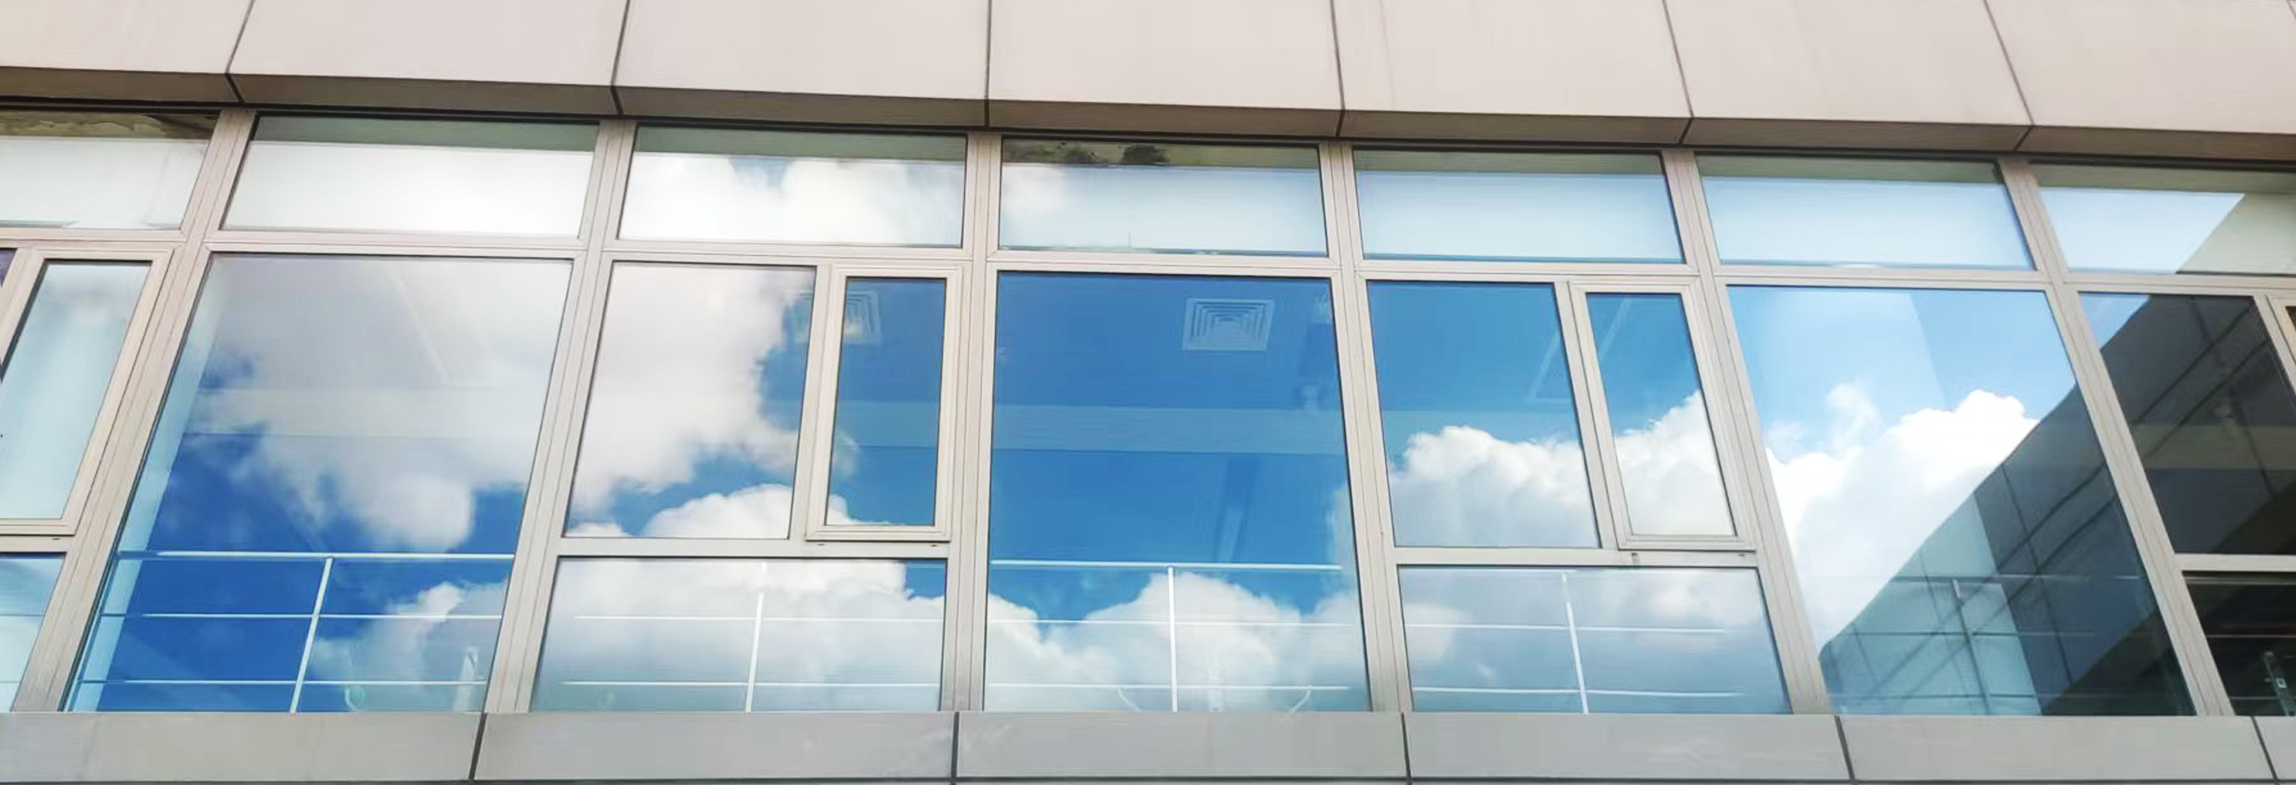
\includegraphics[width=\textwidth]{SKy.png}\\[1.2cm]
  \textbf{Seminar On Algebraic Geometry\\ Lecture Notes 2026 (Draft)}%
}
\author{Zihang Zhang}
\date{}

\begin{document}


\maketitle
\thispagestyle{empty}

\tableofcontents
\newpage

\section{Sheaves}

\subsection{Definitions \& Examples}

Grothendieck's creature in algebraic geometry arises much from 
differential geometry. Roughly speaking, Grothendieck generalized 
both differential geometry and algebraic geometry, in order to provide 
a new geometric view with algebraic objects. 

\begin{definition}
    Let $(X,\mathcal{T})$ be a topology space. 
    A \textbf{presheaf} $\mathscr{F}$ of  category $\mathcal{C}$ 
    is a contravariant functor 
    $$\mathscr{F}: \mathsf{Top}(X) \to \mathscr{C},$$
    where $\mathrm{Top}(X) = (\mathcal{T}, \subseteq)$ 
    is a preorder category. 
    
    In other words, if $\mathscr{F}$ is a presheaf of $\mathrm{Ab}$, 
    then for every open subset $U$ of $X$, 
    there is an abelian group $\mathscr{F}(U)$ and for every 
    inclusion $U \subseteq V$ of open subsets of $X$, 
    there is a morphism of abelian groups 
    $\rho_{VU} = \operatorname{res}_{V,U} : \mathscr{F} (V) \to \mathscr{F} (U)$. 
    And it satisfies
    \begin{enumerate}[label=(\arabic*)]
        \item $\mathscr{F}(\varnothing) = 0$; (Not necessary)
        \item $\rho_{UU}=\operatorname{id}_{U}:\mathscr{F}(U) \to \mathscr{F}(U)$; 
        \item If $U \subseteq V \subseteq W$ are three open subsets, 
        then $\rho_{WU}=\rho_{WV}  \circ \rho_{VU}$. 
    \end{enumerate}

    \begin{center}
        \begin{tikzcd}
            U \arrow[r] \arrow[d,hook] & \mathscr{F}(U) \\
            V \arrow[r] &  \mathscr{F}(V) \arrow[u,"\rho_{VU}"']
        \end{tikzcd}
    \end{center}

    As a matter of terminology, if : $\mathscr{F}$ is a presheaf on $X$, 
    we refer to: $\mathscr{F} ( U)$ as the \textbf{sections} of 
    the presheaf $\mathscr{F}$ over the open set $U$, 
    and we sometimes use the notation $\Gamma(U,\mathscr{F})$ 
    to denote the group $\mathscr{F}(U)$. 
    We call the maps $\rho_{VU}= \operatorname{res}_{V,U}$ 
    \textbf{restriction maps}, and we sometimes 
    write $s\mid_{V}$ instead of $\rho_{VU}(s)$, 
    if $s \in \mathscr{F}(U)$. 

    We always assume that $ \mathcal{C} $ be 
    $ \mathsf{Ab} $, i.e., the category of abelian groups, 
    in order to give the category of presheaves the abelian 
    category structure. 
\end{definition}

Simply, a presheaf is just a contravariant functor 
$ \mathscr{F} : \mathcal{D} \to \mathcal{C} $. 
A sheaf is a presheaf whose sections are, 
in a technical sense, uniquely determined by their restrictions, 
via "glueing together". 

\begin{definition}
    A presheaf $\mathscr{F}$ on a topological space $X$ 
    is a \textbf{sheaf} if it satisfies the following 
    supplementary conditions:
    \begin{enumerate}[label=(\arabic*)]
        \setcounter{enumi}{3}
        \item \textbf{Identity axiom:} 
            If $U$ is an open subset, 
            if $\{V_{i}\}$ is an open covering of $U$, 
            and if $s \in \mathscr{F}(U)$ is an element such 
            that $s \mid_{V_{i}}=0$ for all $i$, 
            then $s=0$. 
            It is equivalent with that  
            $s \mid_{V_{i}}=t\mid_{V_{i}} \implies s=t$. 

        \item \textbf{Glueing axiom:} If $U$ is an open subset, 
        if $\{V_{i}\}$ is an open covering of $U$, 
        and if we have elements $s_{i} \in \mathscr{F}(V_{i})$ 
        for each $i$, with the property that for each $i,j$, 
        $s_{i} \mid_{V_{i}\cap V_{j}}=s_{j} \mid_{V_{i}\cap V_{j}}$ 
        then there is an (by (4), unique) element 
        $s \in \mathscr{F}(U)$ such that $s \mid_{V_{i}} =s_{i}$ 
        for each $i$. 
    \end{enumerate}
\end{definition}

\begin{lemma}
    Let $ \mathscr{F} $ be a sheaf on a topological space $ X $. 
    If $ U $ and $ V $ are disjoint open subsets of $ X $, 
    then $ \mathscr{F}(U \amalg V) \cong \mathscr{F}(U) \times \mathscr{F}(V) $. 
\end{lemma}

\begin{proof}
    The isomorphism is given by $ s \mapsto (s \mid_{U}, s \mid_{V}) $, 
    and the inverse is given by $ (s_{1},s_{2}) \mapsto s$, 
    where $ s $ is glued by $ s_{1} $ and $ s_{2} $, 
    since $ \{U,V\} $ is naturally an open cover of $ U \amalg V $. 
\end{proof}

\begin{example}
    \label{eg: constant sheaf}
    \cite[Exercise II.1.1]{hartsAG}
    Let $A$ be an abelian group (resp., ring), and define the \textbf{constant presheaf} 
    $\underline{A}_{\mathrm{pre}}$ associated to $A$ on the 
    topological space $X$ to be the presheaf 
    $U \mapsto A$ for all $U \neq \varnothing$, 
    with restriction maps the identity. 
    In particular, the constant presheaf $\underline{\mathbb{Z}}_{\mathrm{pre}}$ 
    associated to $\mathbb{Z}$ is given by $U \mapsto \mathbb{Z}$, 
    and any section $s \in \underline{\mathbb{Z}}_{\mathrm{pre}}(U)$ 
    is an integer $s \in \mathbb{Z}$. 

    \cite[Example II.1.0.3]{hartsAG} 
    Let $X$ be a topological space, and $A$ an abelian group (resp., ring). 
    We define the \textbf{constant sheaf} $\underline{A}$ on $X$ determined 
    by $A$ as follows. 

    Give $A$ the discrete topology, and for any open set 
    $U \in X$, let $\underline{A} (U)$ be the group (resp., ring) of all 
    continuous maps of $U$ into $A$: 
    $$\underline{A}(U):=C(U,A).$$ 
    The restriction maps are the usual restrictions 
    of maps. Since $ A $ is a discrete topological group (resp., ring), 
    each $ \underline{A}(U) $ is endowed with group (resp., ring) structure. 
    Immediately, $ \underline{A} $ is an abelian group sheaf (resp., ring) on $ X $. 

    Note that for every connected open set $U$, 
    $\underline{A} (U) \cong A$, whence the name "constant sheaf". 
    To see this, let $s \in \underline{A}(U)$ be a section, 
    then $U=\bigcup_{a \in A} s^{-1}(a)$. 
    Since $U$ is connected, there is only one $s^{-1}(a)=U$ 
    and the others are empty. 
    Thus, we obtain a surjective homomorphism below 
    $$\underline{A}(U) \to A \quad\text{with}\quad s \mapsto s(x),\, \forall x \in U. $$ 
    It is also injective, since $ s(U)=\{0\} $ if and only if 
    $ s =0 $. 

    Therefore, if $ U $ is an open set whose connected components 
    are open, then $ \underline{A}(U)= \prod A $, 
    one for each connected components of $ U $. 

\end{example}

Here we define sheaves of modules in order to take a 
more geometric viewpoint on sheaves. 
They are studied in \cite[II.5 Sheaves of Modules]{hartsAG}.

\begin{definition}
    A \textbf{ringed space} is a pair $ (X,\mathscr{O}_{X}) $ 
    consisting of a topological space $ X $ and a sheaf of rings 
    $ \mathscr{O}_{X} $ on $ X $. 
\end{definition}

\begin{definition}
    Let $ (X,\mathscr{O}_{X}) $ be a ringed space. 
    A \textbf{sheaf of $ \mathscr{O}_{X} $-modules } is a sheaf 
    $ \mathscr{F} $ on $ X $, such that for each open set $ U \subseteq X $, 
    the abelian group $ \mathscr{F}(U) $ is an $ \mathscr{O}_{X} $-module, 
    and for for each inclusion of open sets $ V \subseteq U $, 
    the restriction homomorphism $ \mathscr{F}(U) \to \mathscr{F}(V) $ 
    is compatible with the module structure via the ring homomorphism 
    $ \mathscr{O}_{X}(U) \to \mathscr{O}_X(V) $, that is, 
    for any $ a \in \mathscr{O}_{X}(U) $ and $ s \in \mathscr{F}(U) $, 
    we have $ (a \cdot s)\mid_{V} = (a\mid_{V}) \cdot (s \mid_{V}) $. 
\end{definition}

Far from being abstract nonsense, 
sheaf theory generalizes and unifies many geometric objects. 
Here are some examples from geometry and analysis. 

\begin{example}
Let \(X\) be a topological space. For each open subset \(U\subseteq X\), 
let \(C(U)\) denote the \(\mathbb{R}\)-algebra of continuous functions 
\(U\to \mathbb{R}\), with restriction maps given by restriction of functions. 
Then \(\mathscr{C}\), defined by \(\mathscr{C}(U)=C(U)\), is a sheaf of 
\(\mathbb{R}\)-algebras on \(X\); the glueing axiom follows from the local 
nature of continuity. In particular, if \(M\) is a smooth manifold, then the 
structure sheaf \(\mathscr{O}_{M}\) is the sheaf of smooth functions, given by
\[
\mathscr{O}_{M}(U)=C^{\infty}(U).
\]
\end{example}

\begin{example}
Let \(X\) be a complex manifold. For each open subset \(U\subseteq X\), 
let \(\mathcal{O}(U)\) denote the \(\mathbb{C}\)-algebra of holomorphic 
functions \(U\to \mathbb{C}\), with restriction maps given by restriction 
of functions. Then the structure sheaf \(\mathscr{O}_X\), defined by 
\(\mathscr{O}_X(U)=\mathcal{O}(U)\), is a sheaf of \(\mathbb{C}\)-algebras 
on \(X\): if \(\{U_i\}\) is an open cover of \(U\) and 
\(f_i\in\mathcal{O}(U_i)\) agree on all overlaps \(U_i\cap U_j\), then 
there is a unique \(f\in\mathcal{O}(U)\) restricting to each \(f_i\), 
since holomorphicity is a local property. This is the holomorphic analogue 
of the sheaf of smooth functions on a smooth manifold. 

Already here one sees why one works with sheaves rather than only global 
sections: on a compact connected complex manifold \(X\), every global 
holomorphic function is constant, so \(\mathscr{O}_X(X)\cong\mathbb{C}\), 
whereas the sheaf \(\mathscr{O}_X\) still encodes rich local holomorphic data.
        \item Let \(M\) be a smooth manifold. For each open subset \(U\subseteq M\), let
\(\Omega^k(U)\) denote the \(C^\infty(U)\)-module of smooth \(k\)-forms on
\(U\), with restriction maps given by restriction of forms. Then
\(\Omega^k\) is a sheaf of \(C^\infty_M\)-modules on \(M\). 

Crucially, \(\Omega^k\) is not merely a
sheaf of abelian groups: for \(f\in C^\infty_M(U)\) and
\(\omega\in\Omega^k(U)\), the product \(f\omega\) is defined pointwise by
\((f\omega)_p=f(p)\omega_p\), and restriction is compatible with this
structure, making \(\Omega^k\) a sheaf of modules over the structure sheaf
\(\mathscr{O}_{M}\). In particular, \(\Omega^0=\mathscr{O}_{M}\), and \(\Omega^1\) is
the sheaf of sections of the cotangent bundle \(T^*M\). 

Indeed, sheaves of modules provide an analogue of fibre bundles 
in algebraic geometry.
For example, $ \Omega^{k} $ is a $ \mathscr{O}_{M} $-module, 
and is locally free of rank $ \binom{n}{k}$ over $ \mathscr{O}_{M} $,  
hence corresponds to the vector bundle \(\bigwedge^k T^*M\), 
i.e., $ \Omega^{k} = (-,\bigwedge^k T^*M) $. 

There is a deep relation between sheaves of modules with bundles. 
For example, in differential geometry, the Swan-Serre theorem states
that: 
for $ X $ a smooth manifold with $ \mathbb{R} $-algebra of 
smooth functions $ C^{\infty}(X) $, there is an equivalence of 
categories between that of finite rank smooth vector bundles over $ X $ 
and finitely generated projective modules over $ C^{\infty}(X) $. 
See \cite[Chapter 12]{nes} for more details. 
\end{example}

\begin{example}
Let \(p:Y\to X\) be a continuous map. For each open subset \(U\subseteq X\),
define
\[
\Gamma(Y/X)(U)=\{s:U\to Y \mid p\circ s=\mathrm{id}_U,\ s\text{ continuous}\},
\]
with restriction maps given by \(s\mapsto s|_V\). Then \(\Gamma(Y/X)\) is a
sheaf on \(X\), called the \emph{sheaf of sections} of \(p\). 

If \(p: Y \to X\) is a vector bundle, then \(\Gamma(Y/X)(U)\) is a
\(C^\infty(U)\)-module, and \(\Gamma(Y/X)\) is a sheaf of
\(C^\infty_X\)-modules, locally free of rank equal to the rank of the bundle.
Indeed, the name "section" comes from such sections 
in differential geometry. 
    
\end{example}


\begin{example}
    Let $ M $ be a smooth manifold, for any open subset $ U \subseteq X $, 
    define $ C_{c}^{\infty}(U) $ be the $ \mathbb{R} $-vector space of 
    smooth functions from $ U $ to $ \mathbb{R} $ with compact support. 
    Then $ C_{c} $ forms a presheaf, which is not a sheaf in general. 

    For example, let $ M= \mathbb{R} $, 
    $ \varphi $ be a bump function such that 
    $ \operatorname{supp}(\varphi) = [-1/3,1/3]$, and 
    $ \varphi(0)=1 $. Let 
    $ f(x)= \sum_{n \in \mathbb{Z}} \varphi(x-n) $. 
    Then $ \operatorname{f}(\varphi) = \bigcup_{n \in \mathbb{Z}} [n-1/3,n+1/3] $, 
    hence $ f \notin C_{c}(\mathbb{R}) $. 
    Now let $ U_{n}:=(n-1/2,n+2/3) $ be some open subsets covering $ \mathbb{R} $. 
    In each $ U_{n} $, 
    $\operatorname{supp}(f \mid_{U_{n}})=[n-1/3,n+1/3]$ which is compact. 
    However, the global section glueing by $ f\mid_{U_{n}} $ 
    is identically $ f $, which is not in $ C_{c}^{\infty}(\mathbb{R})$. 

    An interesting result is, as the dual topological space of 
    $ C_{c}^{\infty}(U) $, the space of distributions 
    $ \mathcal{D}'(U) $ forms a sheaf. 
    For a brief introduction to this, see \cite[{4.5}]{wikiDistribution}.
\end{example}

Now we come back to classical algebraic geometry. 
In \cite[I.3 Morphisms]{hartsAG}, we define the ring of regular functions on 
an algebraic variety $ V $, denoted by $ \mathscr{O}(V) $. 

\begin{example}
    \cite[Example II.1.0.1]{hartsAG} 
    Let $ V $ be an algebraic variety over the field $ k $. 
    For each open set $ U \subseteq V $, let 
    $ \mathscr{O}_{V}(U):=\mathscr{O}(U) $ be the ring of regular 
    functions from $ U $ to $ k $. Then $ \mathscr{O}_{V} $ 
    is a presheaf of rings on $ X $. 
    
    $ \mathscr{O}_{V} $ is a sheaf, which is called 
    the \emph{sheaf of regular functions} on $ X $. 
    This is because the regularity of a function is defined locally. 
\end{example}

Now we define the morphisms between presheaves on the same space. 

\begin{definition}
    For a presheaf $\mathscr{F}$ is a contravariant functor 
    $\mathscr{F}: \mathsf{Top}(X) \to \mathsf{Ab}$, 
    it forms a functor category 
    $[\mathsf{Top}(X)^{\mathsf{op}},\mathsf{Ab}]$. 
    We define the category of presheaves as 
    $\mathsf{PSh}(X)=[\mathsf{Top}(X)^{\mathrm{op}},\mathsf{Ab}]$. 
    In general, we define $\mathsf{PSh}(X,\mathcal{C})=[\mathsf{Top}(X)^{\mathrm{op}},\mathcal{C}]$, 
    for any category $ \mathcal{C} $. 

    Thus, the morphism $\varphi: \mathscr{F} \to \mathscr{G}$ 
    is a natural transformation, 
    which consists of morphisms of abelian groups 
    $\varphi(U): \mathscr{F}(U) \to \mathscr{G}(U)$ 
    for each open set $U$, such that whenever 
    $V \subseteq U$ is an inclusion, the diagram 
    \begin{center}
        \begin{tikzcd}
\mathscr{F}(U) \arrow[r, "\varphi(U)"] \arrow[d, "\rho_{UV}"] & \mathscr{G}(U) \arrow[d, "\rho_{UV}"] \\
\mathscr{F}(V) \arrow[r, "\varphi(V)"]                        & \mathscr{G}(V)  
        \end{tikzcd}
    \end{center}
    commutes. Or we can simply say that $ \varphi(s \mid_{V})=\varphi(s)\mid_{V} $, 
    for any section $ s \in \mathscr{F}(U) $. 

    We can simply define the category of sheaves on $ X $ 
    to be the full subcategory $ \mathsf{Sh}(X):=\mathsf{Sh}(X,\mathsf{Ab}) $ of $ \mathsf{PSh}(X) $. 
\end{definition}

\begin{definition}
    Let $\varphi: \mathscr{F} \to \mathscr{G}$ be a morphism of presheaves. 
    We define the presheaf kernel of $\varphi$, 
    presheaf cokernel of $\varphi$, and presheaf image 
    of $\varphi$ to be the presheaves given by 
    $U \mapsto \mathrm{ker}\,\varphi(U)$, 
    $U \mapsto \mathrm{coker}\,\varphi(U)$, 
    and $U \mapsto \mathrm{im}\,\varphi(U)$ respectively. 
\end{definition}

Indeed, $ \mathsf{PSh} $ is an abelian category. 
We denote the cokernel of $ \varphi $ in $ \mathsf{PSh} $ by 
$ \operatorname{coker}_{\mathsf{PSh}} \varphi $ and the image of $ \varphi $ in $ \mathsf{PSh} $ by 
$ \operatorname{im}_{\mathsf{PSh}} \varphi $, 
since they are not sheaves in general. 
However, the kernel of $ \varphi $ in $ \mathsf{PSh} $ is a sheaf, 
by the lemma below. 

\begin{lemma}
    If $\varphi: \mathscr{F} \to \mathscr{G}$ is a morphism 
    of sheaves, then the presheaf kernel of $\varphi$, 
    $\mathrm{ker}\,\varphi$ is also a sheaf. 
\end{lemma}

\begin{proof}
    Notice that $ (\ker \varphi) (U)  \subseteq \mathscr{F}(U) $ 
    hence we can use the sheaf axiom on $ \mathscr{F} $. 
\end{proof}

\subsection{Stalks \& Germs}

Before we investigate the category of sheaves and operations on 
sheaves, we first introduce the stalks of sheaves. 

\begin{definition}[Stalks]
    If $\mathscr{F}$ is a presheaf on $X$, and if $P$ is a point 
    of $X$, we define the \emph{stalk} $\mathscr{F}_{P}$ of 
    $\mathscr{F}$ at $P$ to be the direct limit (colimit) 
    of the groups $\mathscr{F}(U)$ for all open sets $U$ 
    containing $P$, via the restriction maps 
    $\rho$, as 
    $$\mathscr{F}_{P}:= \varinjlim \mathscr{F}(U).$$
    The direct limit means that, for any open neighborhood $ U $ 
    of $ P $, there exists a homomorphism 
    $ \rho_{U} : \mathscr{F}(U) \to \mathscr{F}_{P}$, 
    such that, for compatible homomorphisms $ \lambda_{U}: \mathscr{F}(U) \to A $, 
    there exists a unique homomorphism $ \mathscr{F}_{P} \to A $. 

    Elements in $ \mathscr{F}_{P} $ are called 
    \emph{germs} of sections of $ \mathscr{F} $ at the point $ P $. 

    In fact, the index category $\mathsf{Top}_{P}(X)$ 
    with all open neighborhood $U$ of $P$ is 
    a \emph{filtered category}, since for any open neighborhood 
    $ U $ and $ V $ of $ P $, $ U \cap V $ is also an open 
    neighborhood of $ P $. 
    By \cite[1.4 D]{vakilTheRisingSea}, 
    the germ in $\mathscr{F}_{P}$ has the form of $\langle U,s \rangle$ 
    while $ U $  is the open neighborhood of $P$ and 
    $s \in \mathscr{F}(U)$ under the equivalence relation
     that 
    $$\langle U,s \rangle = \langle V,t \rangle \Longleftrightarrow 
    \,\,\exists\text{ an open neighborhood }W\subseteq U \cap V 
    \text{ of }P \text{ s.t. } s\mid_{W}=t\mid_{W}.$$ 
\end{definition}

In fact, taking stalks gives a functor $ \mathsf{Sh}(X) \to \mathsf{Ab}$, 
which is exact and left-adjoint. 

\begin{example}
    Let $X$ be a complex manifold and let $\mathscr{O}_{X}$ 
    be the sheaf of holomorphic functions on $X$. 
    If $\dim_{\mathbb{C}} X = n$ and $z_1,\dots,z_n$ are local 
    holomorphic coordinates centered at $P \in X$, then the germ of a 
    holomorphic function is uniquely determined by its Taylor 
    expansion at $P$. Hence
    $$\mathscr{O}_{X,P} \cong \mathbb{C}\{z_1,\dots,z_n\},$$
    the ring of convergent power series in $n$ variables. 
    This stalk is a local ring, whose maximal ideal consists of 
    germs vanishing at $P$.
\end{example}

\begin{example}
    The name of germs came from analytic continuation. 
    See \cite[Chapter 8]{ahlfors}.
    
    A \emph{function element} is a pair $(D,f)$ consisting of an open
    disk $D \subset \mathbb{C}$ and a holomorphic function $f$ on $D$.
    Two function elements $(D,f)$ and $(E,g)$ define the same
    \emph{germ} at $z_0 \in D \cap E$ if $f = g$ in a neighborhood of $z_0$.
    The set of all such germs, denoted $\mathcal{O}$, carries a natural
    topology: for each function element $(D,f)$, the collection
    $\{[f]_z : z \in D\}$ is a basic open neighborhood of each of its
    germs. The projection
    $$\pi:\mathcal{O}\to\mathbb{C}, \qquad [f]_z \mapsto z,$$
    is then a local homeomorphism, because the map
    $z \mapsto [f]_z$ is a homeomorphism from $D$ onto
    $\{[f]_z : z \in D\}$ with inverse $\pi$.
    Thus $\mathcal{O}$ is a one-dimensional complex manifold, i.e. a
    Riemann surface, and $\pi$ is holomorphic.
    Its connected components are the Riemann surfaces of the
    \emph{global analytic functions} obtained by analytic continuation:
    continuing a germ $[f]_a$ along a curve $\gamma$ from $a$ to $b$
    amounts to lifting $\gamma$ to $\mathcal{O}$, so the continuation
    becomes a single-valued holomorphic function on the component
    containing $[f]_a$.
\end{example}

\begin{example}
    More generally, let $X$ be a topological space. An
    \emph{\'etale space} over $X$ is a continuous map
    $\pi:\mathcal{F}\to X$ which is a local homeomorphism.
    The fiber $\mathcal{F}_x = \pi^{-1}(x)$ is the \emph{stalk} at $x$.
    If each stalk carries the structure of an abelian group and the
    group operations are continuous, this is the old-fashioned
    definition of a \emph{sheaf of abelian groups} on $X$; the
    sections over an open set $U$ are the continuous maps
    $s:U\to \mathcal{F}$ with $\pi \circ s = \mathrm{id}_U$.
    The modern sheaf $\mathscr{F}$ associated with an \'etale space
    is obtained by taking all sections over open subsets.
\end{example}

\subsection{Local Nature of Sheaves I}

\begin{lemma}
    \label{lemma: taking stalks}
    For every $P \in U$, there is a map 
    $\mathscr{F}(U) \to \mathscr{F}_{P}$, 
    sending a section $s \in \mathscr{F}(U)$ to 
    the equivalence class of $(U,s)$, denoted $s_{P}$. 

    If $\mathscr{F}$ is a sheaf, 
    a section $s \in \mathscr{F}(U)$ of $\mathscr{F}$ over $U$ 
    is determined by its images in the stalks $\mathscr{F}_{x}$ 
    for all $x \in U$, i.e. $s=0$ if and only if 
    $s_{P}=0$, for all $P \in U$. 
    Equivalently, $s=t \in \mathscr{F}(U)$ 
    if and only if $s_{P}=t_{P} \in \mathscr{F}_{P}$, 
    for all $P \in U$.
\end{lemma}

\begin{proof}
    For any germ $ (s_{P},U_{P}) $, such that $ S_{P}=0 $, 
    we can obtain the zero section by glueing $ s_{P} $, 
    since $ U_{P} $ forms an open cover of $ X $. 
    By the identity axiom, any section glueing by $ s_{P} $ 
    must be zero. 
\end{proof}

\begin{proposition}
    \label{prop: injective morphisms}
    \cite[2.4 N]{vakilTheRisingSea}, \cite[Exercise II.1.3]{hartsAG} 
    Consider the morphism $\varphi:\mathscr{F} \to \mathscr{G}$ 
    of sheaves on the topology space $X$. 
    Then, the conditions below are equivalent: 
    \begin{enumerate}[label = (\arabic*)]
    \item $\varphi$ is a monomorphism. 
    \item $\varphi$ is injective on the level 
        of stalks: $\varphi_{P}:\mathscr{F}_{P}\to \mathscr{G}_{P}$ 
        is injective for all $P \in X$. 
    \item $\mathrm{ker}\,\varphi=0$.  
    \item $\varphi$ is injective on the level of open 
    sets : $\varphi(U): \mathscr{F}(U) \to \mathscr{G}(U)$ 
    is a monomorphism of $\mathrm{Ab}$, 
    thus injective and $\mathrm{ker}\,\varphi(U) = (0)$, 
    for all open set $U \subseteq X$. 
    \end{enumerate}

    We say that $\varphi$ is \emph{injective} 
    if it satisfies the above equivalent conditions.
\end{proposition}

\begin{proof}
    We prove this by $(2) \Longrightarrow (1) \Longrightarrow (3) \Longrightarrow (4) \Longrightarrow (2)$. 

    $ (2) \implies (1) $ : By \ref{lemma: taking stalks}. 

    $ (1) \implies (3)$ : By the definition of $\mathrm{ker}\,\varphi$ 
    we could obtain an inclusion morphism 
    $i : \mathrm{ker}\,\varphi \to \mathscr{F}$ 
    and a zero morphism $0:\mathrm{ker}\,\varphi \to \mathscr{F}$ 
    sending $(\mathrm{ker}\,\varphi)(U) \mapsto (0)$ 
    inducing the commutative diagram below 
    \begin{center}
        \begin{tikzcd}
    {\mathrm{ker}\, \varphi} \arrow[r,shift left,"i"] \arrow[r,shift right,"0"'] & \mathscr{F} \arrow[r,"\varphi"] & \mathscr{G}.
    \end{tikzcd}
    \end{center}
    Since $ \varphi $ is a monomorphism, $ i $ must be $ 0 $, 
    which means that $ \ker \varphi = 0 $. 

    $ (3) \implies (4) $ : 
    Notice that $ \ker (\varphi(U))= (\ker \varphi)(U) $. 

    $ (4) \implies (2) $ :
    If $ \ker \varphi(U) = (0) $ for all open sets $ U \subseteq X $, 
    then for any $ P \in X $, and germs $ s_{P} \in \ker \varphi_{P} $, 
    there exists an open neighborhood $ U $ of $ P $, 
    such that $ s_{P} = \langle U, s \rangle $ for some $ s \in \ker \varphi(U) $. 
    By the assumption, $ s = 0 $, hence $ s_{P} = 0 $. 

\end{proof}

Since $ \im_{\mathsf{PSh}} $ is not a sheaf in general, 
the case of epimorphisms is more complicated. 
We need to introduce the sheafification of presheaves, 
in order to obtain the image of a morphism of sheaves. 

\subsection{Sheafification}

\begin{proposition}
    \cite[Proposition II.1.2]{hartsAG}
    Given a presheaf \(\mathscr{F}\), there is a sheaf
    \(\mathscr{F}^{\sh}\) and a morphism
    \(\sh:\mathscr{F}\to\mathscr{F}^{\sh}\)
    with the following universal property: for any sheaf \(\mathscr{G}\)
    and any morphism of presheaves
    \(\varphi:\mathscr{F}\to\mathscr{G}\)
    (where \(\mathscr{G}\) is regarded as a presheaf),
    there is a unique morphism of sheaves
    \(\psi:\mathscr{F}^{\sh}\to\mathscr{G}\)
    such that \(\varphi=\psi\circ\sh\).

    \begin{center}
    \begin{tikzcd}
        \mathscr{F} \arrow[r,"\sh"] \arrow[dr,"\varphi"'] 
        & \mathscr{F}^{\sh} \arrow[d,dashed,"\exists ! \psi"] \\
        & \mathscr{G}
    \end{tikzcd}
    \end{center}

    Furthermore the pair \((\mathscr{F}^{\sh},\sh)\)
    is unique up to a unique isomorphism.
    We call \(\mathscr{F}^{\sh}\) \emph{the sheaf associated to the presheaf}
    \(\mathscr{F}\), or \emph{the sheafification of} \(\mathscr{F}\).
\end{proposition}

\begin{proof}
    We construct the sheafification \(\mathscr{F}^{\sh}\) as follows.
    For any open subset \(U\), let \(\mathscr{F}^{\sh}(U)\) be the set
    of functions
    \[
        s: U \longrightarrow \coprod_{P \in U} \mathscr{F}_{P}
    \]
    such that
    \begin{enumerate}[label = (\arabic*)]
        \item for each \(P \in U\), \(s(P) \in \mathscr{F}_{P}\), and
        \item for each \(P \in U\), there is an open neighborhood
        \(V \subseteq U\) of \(P\), and an element
        \(t \in \mathscr{F}(V)\), such that for all \(Q \in V\),
        the germ \(t_{Q}\) of \(t\) at \(Q\) is equal to \(s(Q)\).
    \end{enumerate}

    By construction, \(\sh\) is naturally defined by sending
    \(s \in \mathscr{F}(U)\) to the function \(P \mapsto s_{P}\).
    The restriction maps are defined by restricting the domain of
    these functions.

    We now verify that \(\mathscr{F}^{\sh}\) is a sheaf.
    For the identity axiom, let \(U \subseteq X\) be open, let
    \(\{U_{i}\}\) be an open cover of \(U\), and let
    \(s \in \mathscr{F}^{\sh}(U)\) satisfy
    \(s|_{U_{i}} = 0\) for all \(i\).
    Since the restriction maps are restrictions of functions,
    \(s|_{U_{i}}(P) = s(P)\) for every \(P \in U_{i}\).
    Given \(P \in U\), choose \(i\) with \(P \in U_{i}\).
    Then
    \[
        s(P) = s|_{U_{i}}(P) = 0.
    \]
    Hence \(s = 0\).

    For the glueing axiom, suppose we are given sections
    \(s_{i} \in \mathscr{F}^{\sh}(U_{i})\) such that
    \[
        s_{i}|_{U_{i} \cap U_{j}}
        =
        s_{j}|_{U_{i} \cap U_{j}}
    \]
    for all \(i,j\). Define
    \(s: U \to \coprod_{P \in U} \mathscr{F}_{P}\) by
    \(s(P) = s_{i}(P)\) whenever \(P \in U_{i}\).
    This is well defined by the compatibility on overlaps.
    To see that \(s \in \mathscr{F}^{\sh}(U)\), fix \(P \in U\)
    and choose \(i\) with \(P \in U_{i}\).
    Since \(s_{i} \in \mathscr{F}^{\sh}(U_{i})\), there is an open
    neighborhood \(V \subseteq U_{i}\) of \(P\) and an element
    \(t \in \mathscr{F}(V)\) such that
    \(t_{Q} = s_{i}(Q)\) for all \(Q \in V\).
    Then \(t_{Q} = s(Q)\) for all \(Q \in V\), so the local
    condition holds at \(P\). Thus \(s \in \mathscr{F}^{\sh}(U)\),
    and \(s|_{U_{i}} = s_{i}\) for every \(i\), because the two
    functions agree at each point of \(U_{i}\).
    Therefore \(\mathscr{F}^{\sh}\) is a sheaf.

    Now we prove the universal property.
    Let \(\varphi:\mathscr{F}\to\mathscr{G}\) be a morphism of
    presheaves, with \(\mathscr{G}\) a sheaf.
    Let \(s \in \mathscr{F}^{\sh}(U)\).
    For each \(P \in U\), by the construction of
    \(\mathscr{F}^{\sh}\), there is an open neighborhood
    \(V_{P} \subseteq U\) of \(P\) and an element
    \(t^{P} \in \mathscr{F}(V_{P})\) such that
    \[
        s(Q) = t^{P}_{Q}
        \qquad
        \text{for all } Q \in V_{P}.
    \]
    We claim that for any \(P,Q \in U\), the sections
    \(\varphi(t^{P})\) and \(\varphi(t^{Q})\) agree on
    \(V_{P}\cap V_{Q}\). Indeed, for every
    \(R \in V_{P}\cap V_{Q}\), we have
    \[
        \varphi_{R}\bigl(t^{P}_{R}\bigr)
        =
        \varphi_{R}\bigl(s(R)\bigr)
        =
        \varphi_{R}\bigl(t^{Q}_{R}\bigr).
    \]
    Thus the germs of \(\varphi(t^{P})\) and \(\varphi(t^{Q})\)
    at every point of \(V_{P}\cap V_{Q}\) coincide.
    Since \(\mathscr{G}\) is a sheaf,
    \autoref{lemma: taking stalks} implies
    \[
        \varphi(t^{P})|_{V_{P}\cap V_{Q}}
        =
        \varphi(t^{Q})|_{V_{P}\cap V_{Q}}.
    \]
    Therefore, by the glueing axiom for the sheaf \(\mathscr{G}\),
    there exists a unique section
    \(\psi(s) \in \mathscr{G}(U)\) such that
    \[
        \psi(s)|_{V_{P}} = \varphi(t^{P})
        \qquad
        \text{for all } P \in U.
    \]
    The section \(\psi(s)\) is independent of the choices of
    \(V_{P}\) and \(t^{P}\): if \(W_{P},u^{P}\) is another choice,
    then on \(V_{P}\cap W_{P}\) the sections
    \(\varphi(t^{P})\) and \(\varphi(u^{P})\) have the same germs
    at every point, hence are equal because \(\mathscr{G}\) is a
    sheaf; uniqueness in the glueing axiom then gives the same
    global section.

    It is immediate from the local description that \(\psi\) is
    compatible with restriction maps, hence \(\psi\) is a morphism
    of sheaves. Moreover, for \(t \in \mathscr{F}(U)\), the section
    \(\psi(\sh(t))\) agrees locally with \(\varphi(t)\), so
    \(\psi\circ\sh = \varphi\).

    Finally, suppose that
    \(\psi':\mathscr{F}^{\sh}\to\mathscr{G}\) is another morphism
    of sheaves such that \(\psi'\circ\sh = \varphi\).
    For \(s \in \mathscr{F}^{\sh}(U)\) and \(P \in U\), using the
    same local data \(V_{P},t^{P}\), we have
    \[
        \psi'(s)|_{V_{P}}
        =
        \psi'(\sh(t^{P}))|_{V_{P}}
        =
        \varphi(t^{P})
        =
        \psi(s)|_{V_{P}}.
    \]
    Since \(\mathscr{G}\) is a sheaf, this implies
    \(\psi'(s)=\psi(s)\). Hence \(\psi'=\psi\).
    The uniqueness of \((\mathscr{F}^{\sh},\sh)\) up to a unique
    isomorphism follows formally from the universal property.
\end{proof}

\begin{lemma}
    \label{lemma: sheafification on stalks}
    \cite[2.4 M]{vakilTheRisingSea}
    The sheafification
    \(\sh:\mathscr{F}\to\mathscr{F}^{\sh}\)
    induces an isomorphism on stalks:
    \[
        \sh_{P}:\mathscr{F}_{P}
        \longrightarrow
        \mathscr{F}^{\sh}_{P},
        \qquad
        \forall P \in X.
    \]

    Conversely, let \(\mathscr{F}\) be a presheaf,
    let \(\mathscr{G}\) be a sheaf, and let
    \(\varphi:\mathscr{F}\to\mathscr{G}\) be a morphism of
    presheaves. If the induced map
    \(\varphi_{P}:\mathscr{F}_{P}\to\mathscr{G}_{P}\)
    is an isomorphism for all \(P \in X\), then the induced
    morphism
    \(\varphi^{\sh}:\mathscr{F}^{\sh}\to\mathscr{G}\)
    is an isomorphism.
\end{lemma}

\begin{proof}
    First we prove that \(\sh_{P}\) is injective.
    Let \(\alpha \in \mathscr{F}_{P}\), and choose a
    representative \(s \in \mathscr{F}(U)\) of \(\alpha\).
    Suppose that \(\sh_{P}(\alpha)=0\).
    Then \(\sh(s)_{P}=0\) in \(\mathscr{F}^{\sh}_{P}\).
    Hence there is an open neighborhood \(V \subseteq U\) of \(P\)
    such that
    \[
        \sh(s)|_{V} = 0
        \qquad
        \text{in } \mathscr{F}^{\sh}(V).
    \]
    For every \(Q \in V\), we have
    \[
        \sh(s)(Q) = s_{Q}.
    \]
    Therefore \(s_{Q}=0\) for every \(Q \in V\).
    In particular, taking \(Q=P\), we obtain \(s_{P}=0\) in
    \(\mathscr{F}_{P}\), that is, \(\alpha=0\).
    Thus \(\sh_{P}\) is injective.

    Next we prove that \(\sh_{P}\) is surjective.
    Let \(\beta \in \mathscr{F}^{\sh}_{P}\), and choose a
    representative
    \(\sigma \in \mathscr{F}^{\sh}(U)\) of \(\beta\).
    By the construction of \(\mathscr{F}^{\sh}\), after possibly
    shrinking \(U\) to an open neighborhood \(V\) of \(P\), there
    exists \(t \in \mathscr{F}(V)\) such that
    \[
        t_{Q} = \sigma(Q)
        \qquad
        \text{for all } Q \in V.
    \]
    Hence \(\sh(t)|_{V} = \sigma|_{V}\), and therefore
    \[
        \sh_{P}(t_{P})
        =
        \sh(t)_{P}
        =
        \sigma_{P}
        =
        \beta.
    \]
    Thus \(\sh_{P}\) is surjective.
    Consequently \(\sh_{P}\) is an isomorphism for every
    \(P \in X\).

    For the converse, the universal property of sheafification
    gives a unique morphism
    \(\varphi^{\sh}:\mathscr{F}^{\sh}\to\mathscr{G}\)
    such that
    \(\varphi^{\sh}\circ\sh = \varphi\).
    On stalks, since \(\sh_{P}\) is an isomorphism, we obtain
    \[
        \varphi^{\sh}_{P}
        =
        \varphi_{P}\circ\sh_{P}^{-1}.
    \]
    By assumption \(\varphi_{P}\) is an isomorphism for every
    \(P \in X\). Hence \(\varphi^{\sh}_{P}\) is an isomorphism
    for every \(P \in X\).
    By \autoref{prop: isomorphism of sheaves},
    \(\varphi^{\sh}\) is an isomorphism.
\end{proof}

\begin{proposition}
    \label{prop: sheafification as a functor}
    \cite[2.4 H]{vakilTheRisingSea}
    Let $\mathscr{F},\mathscr{G} \in \mathrm{PSh}(X)$ be a presheaf of $X$, 
    let $\mathscr{F}^{\mathrm{sh}},\mathscr{G}^{\mathrm{sh}}\in \mathrm{Sh}(X)$ be the sheafification 
    of them. If there is a morphism $\varphi:\mathscr{F} \to \mathscr{G}$, 
    then there exists a (unique) natural induced morphism of sheaves 
    $\varphi^{\mathrm{sh}}: \mathscr{F}^{\mathrm{sh}} \to \mathscr{G}^{\mathrm{sh}}$, 
    such that the following diagram commutes. 
    \begin{center}
        \begin{tikzcd}
\mathscr{F} \arrow[r,"\varphi"] \arrow[d,"\mathrm{sh}"] & \mathscr{G} \arrow[d,"\mathrm{sh}"] \\
\mathscr{F}^{\mathrm{sh}} \arrow[r,"\varphi^{\mathrm{sh}}"] & \mathscr{G}^{\mathrm{sh}} 
\end{tikzcd}
    \end{center}
\end{proposition}

\begin{proof}
    This follows from the universal property of sheafification. 
\end{proof}

\begin{remark}
    Indeed, \autoref{prop: sheafification as a functor} shows that the sheafification is a functor 
    $ \sh : \PSh \to \Sh $. Moreover, it is left-adjoint to the inclusion functor $ \Sh \to \PSh $, 
    i.e., for any presheaf $ \mathscr{F} $ and sheaf $ \mathscr{G} $, 
    $$ \Hom_{\Sh}(\mathscr{F}^{\sh},\mathscr{G}) \cong \Hom_{\PSh}(\mathscr{F},\mathscr{G}). $$
    % 如果有空写 skyscraper sheaf 就把这里加上去一个纯泛性质的证明
\end{remark}

\begin{example}
    Let $ A $ be an abelian group, and $ X $ be a topological space. 
    We have defined the constant presheaf $ \underline{A}_{\operatorname{pre}} $ on $ X $, 
    and the constant sheaf $ \underline{A} $ on $ X $ in \autoref{eg: constant sheaf}. 
    We claim that $ \underline{A} $ is the sheafification of 
    $ \underline{A}_{\operatorname{pre}} $. 
    
    
    Indeed, the natural morphism $ \underline{A}_{\operatorname{pre}} \to \underline{A} $ 
    is the identity on stalks: both stalks are $ A $, since a germ of a 
    locally constant function is constant on a small neighborhood. 
    Hence this morphism is an isomorphism on all stalks, and therefore 
    the induced morphism $ \underline{A}_{\operatorname{pre}}^{\sh} \to \underline{A} $ 
    is an isomorphism on stalks by \autoref{lemma: sheafification on stalks}. 
    It follows that $ \underline{A} $ is the sheafification of 
    $ \underline{A}_{\operatorname{pre}} $. 

    One can check that each sheaves of abelian groups on $ X $ 
    is a $ \underline{\mathbb{Z}} $-sheaves on $ X $ 
    by definition. 
    We will prove this by $ \mathscr{H}om $ in the next time. 
\end{example}

Now we can define the cokernel and image of a morphism of sheaves, 
hence giving a complete description of the abelian category of sheaves. 

\begin{definition}
    Let $\varphi: \mathscr{F} \to \mathscr{G}$ be a morphism of sheaves. 
    \begin{itemize}
        \item We define the kernel of $\varphi$ to be the presheaf kernel of $\varphi$, 
        $ \ker \varphi $. 
        \item We define the cokernel of $\varphi$ to be the sheafification of the presheaf cokernel of $\varphi$, 
    $\operatorname{coker}\,\varphi := (\operatorname{coker}_{\PSh}\,\varphi)^{\sh}.$
        \item We define the image of $\varphi$ to be the sheafification of the presheaf image of $\varphi$, 
    $\operatorname{im}\,\varphi := (\operatorname{im}_{\PSh}\,\varphi)^{\sh}.$ 
    \end{itemize}
\end{definition}

\begin{corollary}
    \cite[Exercise II.1.4]{hartsAG}
    Let $\varphi: \mathscr{F} \to \mathscr{G}$ be an injective morphism of sheaves. 
    Then the induced map $\varphi^{\sh} : \mathscr{F}^{\sh}\to \mathscr{G}^{\sh}$ 
    of sheafifications is injective. 
    Therefore, we can view $\im \varphi$ as a natural subsheaf 
    of $\mathscr{G}$. 
\end{corollary}

\begin{proof}
    We check this on the level of stalks. 
    Notice that $ \varphi^{\sh}_{P} = \sh_{P} \circ \varphi_{P} \circ \sh_{P}^{-1} $ 
    since $ \sh_{P} $ is an isomorphism, by \ref{lemma: sheafification on stalks}. 
    Therefore, $ \varphi^{\sh}_{P} $ is injective for all $ P \in X $, 
    since $ \varphi_{P} $ is injective for all $ P \in X $. 
\end{proof}

\subsection{Local Nature of Sheaves II}

By giving the definition of image in the category of sheaves, 
we can now give an analogue of \autoref{prop: injective morphisms} for epimorphisms. 

\begin{proposition}
    \label{prop: surjective morphisms}
    \cite[2.4 O]{vakilTheRisingSea}, \cite[Ex 1.3]{hartsAG} 
    Consider the morphism $\varphi:\mathscr{F} \to \mathscr{G}$ of sheaves 
    on the topology space $X$. 
    Then, the conditions below are equivalent: 
    \begin{enumerate}[label = (\arabic*)]
        \item $\varphi$ is an epimorphism. 
        \item $\varphi$ is surjective on the level of stalks: 
        $\varphi_{P}:\mathscr{F}_{P}\to \mathscr{G}_{P}$ is surjective for all $P \in X$. 
    
        \item $\operatorname{im}\,\varphi = \mathscr{G}$. 
        \item For every open set $ U \subseteq X $, 
        and for every section $ s \in \mathscr{G}(U) $, 
        there is a covering $ \{U_{i}\} $ of $ U $, 
        and sections $ t_{i} \in \mathscr{F}(U_{i}) $ 
        such that $ \varphi(t_{i})=s\mid_{U_{i}} $ for all $ i $. 
    \end{enumerate}

    We say that $\varphi$ is \emph{surjective} 
    if it satisfies the above equivalent conditions.
\end{proposition}

\begin{proof}
We prove this by $ (2) \implies (1) \implies (3) \implies (4) \implies (2) $. 
The proof of $ (2) \implies (1) $ and $ (1) \implies (3) $ is similar to \autoref{prop: injective morphisms}. 

$ (3) \implies (4): $ Let $ U $ be an open set, and $ s \in \mathscr{G}(U) $ be a section. 
Since $ \operatorname{im}\,\varphi = \mathscr{G} $, for each $ P \in U $, 
there exists an open neighborhood $ V_{P} \subseteq U $ of $ P $, and a section 
$ t^{P} \in \mathscr{F}(V_{P}) $ such that $ \varphi(t^{P}) = s\mid_{V_{P}} $, 
because of the construction of the sheafification. 
Then $ \{V_{P}\}_{P \in U} $ is an open cover of $ U $, and the sections $ t^{P} $ satisfy 
$ \varphi(t^{P}) = s\mid_{V_{P}} $ for all $ P \in U $. 

$ (4) \implies (2): $ For every point $ P \in X $, and every germ 
$ \langle s, U \rangle \in \mathscr{G}_{P} $, there is a covering $ \{U_{i}\} $ of $ U $ and sections 
$ t_{i} \in \mathscr{F}(U_{i}) $ such that $ \varphi(t_{i})=s \mid_{U_{i}} $, by assumption. 
Choose an open neighborhood $ U_{i} $ of $ P $, then 
$ \langle s,U \rangle = \langle s,U_{i} \rangle =  \langle \varphi(t_{i}),U_{i} \rangle $ 
in $ \mathscr{G}_{P} $. This proves $ \varphi_{P} $ is surjective. 
\end{proof}

\begin{corollary}
    \cite[Exercise II.1.2]{hartsAG} 
    A sequence of sheaves 
    $$ \cdots \to \mathscr{F}^{i-1} \xrightarrow{\varphi^{i-1}} \mathscr{F}^{i} \xrightarrow{\varphi^{i}}\mathscr{F}^{i+1} \to \cdots $$ 
    is exact if and only if the induced sequence of stalks 
    $$ \cdots \to \mathscr{F}^{i-1}_{P} \xrightarrow{\varphi^{i-1}_{P}} \mathscr{F}^{i}_{P} \xrightarrow{\varphi^{i}_{P}}\mathscr{F}^{i+1}_{P} \to \cdots $$ 
    for all $ P \in X $.  
\end{corollary}

\begin{proposition}
    \label{prop: isomorphism of sheaves}
    \cite[Proposition II.1.1]{hartsAG} 
    Let Let $\varphi: \mathscr{F} \to \mathscr{G}$ be a morphism of sheaves on a topological space $X$. 
    Then $\varphi$ is an isomorphism if and only if the 
    induced map on the stalk $\varphi_{P}: \mathscr{F}_{P} \to \mathscr{G}_{P}$ is 
    an isomorphism for every $P \in X$. 
\end{proposition}

\begin{proof}
    By \autoref{prop: injective morphisms} and \autoref{prop: surjective morphisms}. 
\end{proof}

\begin{proposition}
    \cite[Exercise II.1.2]{hartsAG} 
    For any morphism of sheaves $\varphi:\mathscr{F} \to \mathscr{G}$, 
    for each point $P \in X$, $(\mathrm{ker}\,\varphi)_{P}=\mathrm{ker}\,(\varphi_{P})$ 
    and $(\mathrm{im}\,\varphi)_{P}=\mathrm{im}\,(\varphi_{P})$. 
\end{proposition}

\begin{proof}
    Left to readers. 
\end{proof}

% \section{Historical Remark} 有空回来写

\subsection{Abelian Category Of Sheaves}

Let $ X $ be a topological space. 

\begin{definition}
  Let $\mathscr{F}'$ be a subsheaf of a sheaf $\mathscr{F}$, 
  i.e. there is an injective morphism $ i:\mathscr{F}' \to \mathscr{F} $ 
  (we can view $ \mathscr{F}'(U) $ as a subsheaf of $ \mathscr{F}(U) $ for each open subset $ U $). 
  We define the quotient sheaf $\mathscr{F} / \mathscr{F}'$ to be the sheafification 
  of the presheaf $U \mapsto \mathscr{F}(U) / \mathscr{F}'(U)$. 
  For any $ P \in X $, we have $ (\mathscr{F} / \mathscr{F}')_{P} = \mathscr{F}_{P} / \mathscr{F}'_{P} $. 
\end{definition}

\begin{corollary}
  \cite[Exercise II.1.7]{hartsAG}
  Let $\varphi:\mathscr{F} \to \mathscr{G}$ be a morphism of sheaves. 
  Then $\im\varphi \cong \mathscr{F} / \ker \varphi$, and 
  $\mathrm{coker}\,\varphi \cong \mathscr{G} / \mathrm{im}\,\varphi$. 
\end{corollary}

\begin{proposition}[Direct sum]
  \cite[Exercise II.1.9]{hartsAG}
\end{proposition}

\begin{proposition}[Direct limit]
  \cite[Exercise II.1.10, 1.11]{hartsAG}
\end{proposition}

\begin{proposition}[Inverse limit]
  \cite[Exercise II.1.12]{hartsAG}
\end{proposition}



\subsection{Operations on Sheaves}

\subsubsection{Global Section Functor}

Recall that we sometimes write $ \Gamma(U,\mathscr{F}):= \mathscr{F}(U)$, 
for any open subset $ U \subseteq X $ and any sheaf $ \mathscr{F} $ on $ X $. 

\begin{proposition}
  \label{prop: left-exactness of Gamma}
    \cite[Ex 1.8]{hartsAG} 
    Suppose $U \subseteq X$ is an open subset, 
    and $0 \to \mathscr{F} \to \mathscr{G} \to \mathscr{H}$ is an exact sequence 
    of sheaves of abelian groups. 
    Then $$0 \to \Gamma(U,\mathscr{F}) \to \Gamma(U,\mathscr{G}) \to \Gamma(U,\mathscr{H})$$
    is exact. I.e., $ \Gamma(U,-) $  is a left exact functor $\mathrm{Sh}(X) \to \mathrm{Ab}$. 
\end{proposition}

\begin{proof}
  We can easily check this on the level of stalks, 
  since for any morphism $ \varphi: \mathscr{F} \to \mathscr{G} $ of sheaves, 
  and for any $ P \in U $, we have $ \ker \varphi_{P} = (\ker \varphi)_{P} $ and 
  $ \im \varphi_{P} = (\im \varphi)_{P} $.  
\end{proof}

However, $ \Gamma(U,-) $ is not exact in general, especially in algebraic geometry:
a surjective morphism of sheaves need not induce a surjection on sections. 
The following two examples illustrate that differential topology is ``soft,'' 
whereas the Zariski topology is ``hard.'' 

\begin{lemma}
  \label{lemma: partition of units}
  Let $ M $ be a smooth (paracompact) manifold and let $ \{U_{i}\}_{i \in I} $ be an open cover of $ M $. 
  Then there exists a locally finite partition of unity subordinate to $ \{U_{i}\} $: 
  a family $ \{\rho_{i}\}_{i \in I} $ of smooth functions $ \rho_{i} \in C^{\infty}(M) $ such that 
  $ 0 \le \rho_{i} \le 1 $, $ \operatorname{supp}\rho_{i} \subseteq U_{i} $ is compact, 
  the family $ \{\operatorname{supp}\rho_{i}\}_{i \in I} $ is locally finite, and 
  $ \sum_{i \in I} \rho_{i} = 1 $ on $ M $ (the sum is locally finite, hence well defined).
\end{lemma}

\begin{example}
  Let $ M $ be a smooth manifold, $ \mathscr{C}^{\infty}_{M} $ the sheaf of smooth functions on $ M $, 
  and $ \mathscr{C}^{\infty}_{M,c} $ the presheaf of compactly supported smooth functions. 
  The inclusion $ \mathscr{C}^{\infty}_{M,c} \hookrightarrow \mathscr{C}^{\infty}_{M} $ induces an isomorphism 
  $$ (\mathscr{C}^{\infty}_{M,c})^{\sh} \xrightarrow{\sim} \mathscr{C}^{\infty}_{M} $$
  on sheafification. Indeed, for each $ f \in C^{\infty}(M) $ and each point, choose a locally finite open cover 
  $ \{U_{i}\}_{i \in I} $ of $ M $ by relatively compact open subsets and a partition of unity 
  $ \{\rho_{i}\}_{i \in I} $ subordinate to it. Then each $ f_{i} := \rho_{i} f $ is compactly supported 
  and only finitely many $ f_{i} $ are nonzero near each point, so $ f = \sum_{i} f_{i} $ 
  with $ \sum_{i} f_{i} \in \Gamma(M,\mathscr{C}^{\infty}_{M,c}) $. 
  Thus every smooth function is locally a sum of compactly supported smooth functions, 
  and the sheafification of $ \mathscr{C}^{\infty}_{M,c} $ is $ \mathscr{C}^{\infty}_{M} $.
\end{example}

\begin{proposition}
  Let $ M $ be a smooth manifold and $ \mathscr{O}_{M} := \mathscr{C}^{\infty}_{M} $ the sheaf of smooth functions. 
  Then the global section functor 
  $$ \Gamma(M,-) : \mathscr{O}_{M}\text{-}\mathsf{Mod} \longrightarrow \mathsf{Ab} $$
  is exact.
\end{proposition}

\begin{proof}
  Since $ \Gamma(M,-) $ is left exact, it suffices to show that every surjective morphism 
  $ \varphi : \mathscr{F} \to \mathscr{G} $ of $ \mathscr{O}_{M} $-modules induces a surjection on global sections. 
  Let $ g \in \Gamma(M,\mathscr{G}) $. As $ \varphi $ is an epimorphism of sheaves, there exist an open cover 
  $ \{U_{i}\}_{i \in I} $ of $ M $ and local lifts $ f_{i} \in \mathscr{F}(U_{i}) $ with 
  $ \varphi(f_{i}) = g|_{U_{i}} $. Choose a partition of unity $ \{\rho_{i}\}_{i \in I} $ subordinate to 
  $ \{U_{i}\}_{i \in I} $. Since $ \mathscr{F} $ is an $ \mathscr{O}_{M} $-module, the section 
  $ \rho_{i} f_{i} \in \mathscr{F}(U_{i}) $ vanishes near the boundary of $ U_{i} $, hence extends by zero 
  to a global section $ \widetilde{\rho_{i} f_{i}} \in \Gamma(M,\mathscr{F}) $. 
  By local finiteness the sum $ f := \sum_{i \in I} \widetilde{\rho_{i} f_{i}} $ is a well-defined global section of $ \mathscr{F} $, and
  $$ \varphi(f) = \sum_{i \in I} \rho_{i}\,\varphi(f_{i}) = \sum_{i \in I} \rho_{i}\, g|_{U_{i}} = g . $$
  Hence $ \varphi $ is surjective on global sections, and $ \Gamma(M,-) $ is exact.
\end{proof}

\begin{example}
  \cite[Example 2.4.10]{vakilTheRisingSea}
  Let $X=\mathbb{C}$ with the classical topology, 
  and define $\mathscr{O}_{X}$ to be the sheaf of holomorphic functions, 
  and $\mathscr{O}_{X}^{*}$ to be the sheaf of invertible holomorphic functions. 
  Then we have an exact sequence 
  $$0 \xrightarrow{\quad \quad} \underline{\mathbb{Z}} 
  \xrightarrow{\quad \times 2 \pi i \quad} \mathscr{O}_{X} 
  \xrightarrow{\quad \mathrm{exp} \quad} \mathscr{O}_{X}^{*} 
  \xrightarrow{\quad  \quad}1,$$
  where $\underline{\mathbb{Z}}$ is the constant sheaf associated to $\mathbb{Z}$. 

  Indeed, we can check this on stalks. Without loss of generality, consider $ P=0 $/ 
  Then $ \underline{\mathbb{Z}}_{0} = \mathbb{Z} $, 
  and $ \mathscr{O}_{X,0} $ is the ring of convergent Taylor series at origin, 
  and $ \mathscr{O}_{X,0}^{*} $ is the ring of functions in $  \mathscr{O}_{X,0} $ 
  which doesn't vanish at $ 0 $. The image of $ \times 2 \pi i $ on stalks 
  is $ 2 \pi i \mathbb{Z}$ as constant functions, and the kernel of $ \exp $ is just 
  $ 2 \pi i \mathbb{Z} $ by Euler's equation. 
  To show that the expotential map is surjective on stalks, we only need to notice that 
  for any holomorphic function $ f \in \mathscr{O}_{X,0}^{*} $, 
  there is an open neighborhood $ U $ of the origin such that $ f $ has no roots in $ U $. 
  Thus, $ \ln f $ is a holomorphic function in $ U $, which gives the preimage of $ f $ 
  in $ \mathscr{O}_{X,0} $. 

  Let $ U = \mathbb{C} \setminus \{0\} $ be the punctured complex plane. 
  Suppose that there is some $ f \in \mathscr{O}_{X}(U) $, such that 
  $ \exp f = \id_{U} \in \mathscr{O}_{X}^{*}(U)$, i.e., $ \exp(f(z))=z $ on $ U $. 
  Then $ f'(z)z = f'(z) e^{f(z)} = 1 $, for $ z \in U $, and we have $ f'(z) = 1/z $. 
  Now we calculate the integral at 
  $\gamma:|z|=1$: 
  $$\oint_{\gamma} f'(z) \,\mathrm{d}z = \oint_{\gamma} \frac{1}{z} \,
  \mathrm{d}z =2 \pi i  \neq 0.$$
  However, by Cauchy's Integral Theorem, since $\gamma$ is a closed curve 
  containing in $U$, a holomorphic open domain of $f'(z)$, 
  the integral must be zero. 
  Therefore, such $f$ does not exist, and $\exp(U)$ is not surjective. 
\end{example}

\subsubsection{Hom Sheaf}

\begin{proposition}
  \cite[Exercise II.1.15]{hartsAG}
  Let $\mathscr{F},\mathscr{G}$ be sheaves of abelian groups on $X$. 
  For any open set $U \subseteq X$, the set 
  $\mathscr{H}{om}\,(\mathscr{F}\mid_{U},\mathscr{G}\mid_{U})$ 
  is an abelian group, and $\mathscr{H}{om}(\mathscr{F},\mathscr{G})$ 
  is a sheaf of abelian groups on $X$, 
  by $U \mapsto \mathrm{Hom}\,(\mathscr{F}\mid_{U},\mathscr{G}\mid_{U})$. 
  It is called the \emph{sheaf of local morphisms} 
  of $\mathscr{F}$ into $\mathscr{G}$, 
  "sheaf hom" for short, and is denoted $\mathrm{Hom}\,(\mathscr{F},\mathscr{G})$. 
\end{proposition}

\begin{proof}
  For each open $U\subseteq X$, the set $\mathrm{Hom}(\mathscr{F}\mid_U,\mathscr{G}\mid_U)$ becomes an abelian group under pointwise addition: for morphisms $\varphi,\psi$ and any open $V\subseteq U$, $s\in\mathscr{F}(V)$, put
  \[
    (\varphi+\psi)(V)(s)=\varphi(V)(s)+\psi(V)(s),
  \]
  and define $(-\varphi)(V)(s)=-\varphi(V)(s)$, the zero morphism sending every section to $0$. The group axioms are inherited from the abelian groups $\mathscr{G}(V)$, so $U\mapsto\mathrm{Hom}(\mathscr{F}\mid_U,\mathscr{G}\mid_U)$ is a presheaf of abelian groups.

  It remains to check the sheaf axioms. Let $U\subseteq X$ be open and $\{U_i\}_{i\in I}$ an open cover of $U$.
  \emph{Identity:} if $\varphi\in\mathrm{Hom}(\mathscr{F}\mid_U,\mathscr{G}\mid_U)$ satisfies $\varphi|_{U_i}=0$ for all $i$, then for every open $V\subseteq U$ and $s\in\mathscr{F}(V)$ the sections $\varphi(V)(s)|_{V\cap U_i}=0$ for all $i$; since $\mathscr{G}$ is a sheaf and $\{V\cap U_i\}_{i\in I}$ covers $V$, we get $\varphi(V)(s)=0$, hence $\varphi=0$.
  \emph{Gluing:} suppose $\varphi_i\in\mathrm{Hom}(\mathscr{F}\mid_{U_i},\mathscr{G}\mid_{U_i})$ satisfy $\varphi_i|_{U_i\cap U_j}=\varphi_j|_{U_i\cap U_j}$ for all $i,j$. For open $V\subseteq U$ and $s\in\mathscr{F}(V)$, the sections $\varphi_i(V\cap U_i)(s|_{V\cap U_i})\in\mathscr{G}(V\cap U_i)$ agree on the overlaps $V\cap U_i\cap U_j$; by the sheaf property of $\mathscr{G}$ they glue to a unique section $\varphi(V)(s)\in\mathscr{G}(V)$. The assignments $V\mapsto\varphi(V)$ define a morphism of sheaves $\mathscr{F}\mid_U\to\mathscr{G}\mid_U$, and $\varphi|_{U_i}=\varphi_i$ by construction. Hence the presheaf is a sheaf of abelian groups.
\end{proof}

\begin{proposition}
  \cite[Exercise 2.6.I]{vakilTheRisingSea}
  Suppose $\mathscr{F}$ is a sheaf of abelian groups on a topological space $X$. 
  Then $\mathscr{H}{om}\,(\mathscr{F},\cdot)$ is a left-exact functor 
  $\mathrm{Sh}(X) \to \mathrm{Sh}(X)$, a
  nd $\mathscr{H}{om}\,(\cdot,\mathscr{F})$ is a left-exact contravariant 
  functor $\mathrm{Sh}(X) \to \mathrm{Sh}(X)$, as we define above. 
\end{proposition}

\begin{proof}
  Since the Hom sheaf is defined on sections by
  $\mathscr{H}{om}(\mathscr{F},\mathscr{G})(U)=\mathrm{Hom}(\mathscr{F}\mid_U,\mathscr{G}\mid_U)$,
  and exactness of a sequence of sheaves is checked on every open set (restriction to an open subset preserves exactness), it suffices to prove the corresponding exactness of $\mathrm{Hom}$ in $\mathrm{Sh}(U)$ for each open $U$.

  Let $0\to\mathscr{G}'\xrightarrow{\alpha}\mathscr{G}\xrightarrow{\beta}\mathscr{G}''$ be exact. We show that
  \[
    0\to\mathrm{Hom}(\mathscr{F},\mathscr{G}')\xrightarrow{\alpha_*}\mathrm{Hom}(\mathscr{F},\mathscr{G})\xrightarrow{\beta_*}\mathrm{Hom}(\mathscr{F},\mathscr{G}'')
  \]
  is exact. If $\alpha\circ\varphi=0$, then $\varphi=0$ since $\alpha$ is injective; hence $\alpha_*$ is injective. As $\beta\circ\alpha=0$, we have $\beta_*\circ\alpha_*=0$. Conversely, if $\beta\circ\varphi=0$, then $\varphi$ factors through $\ker\beta=\operatorname{im}\alpha\cong\mathscr{G}'$ (using that $\alpha$ is injective), so $\varphi=\alpha\circ\psi$ for a unique $\psi\in\mathrm{Hom}(\mathscr{F},\mathscr{G}')$. Thus $\ker\beta_*=\operatorname{im}\alpha_*$, proving left-exactness of $\mathscr{H}{om}(\mathscr{F},\cdot)$.
\end{proof}


\subsection{Pushforward \& Inverse Image}

\begin{definition}
  Let $f: X \to Y$ be a continuous map of topological spaces.
  \begin{itemize}
    \item For any sheaf $ \mathscr{F} $ on $ X $, we define the \emph{direct image (pushforward)} 
    sheaf $ f_{*}\mathscr{F} $ on $ Y $ by $$ f_{*}\mathscr{F}(V):=\mathscr{F}(f^{-1}V),$$ 
    for any open set $ V \subseteq Y $. 
    \item For any sheaf $ \mathscr{G} $ on $ Y $, we define a  
    presheaf 
    $ f^{+}\mathscr{G} $ on $ X $ by $$ f^{+}\mathscr{G}(U)=
    \varinjlim_{V \supseteq f(U)} \mathscr{G}(V),$$ 
    for any open set $ U \subseteq X $. And we define \emph{inverse image} 
    sheaf $ f^{-1}\mathscr{G} $ to be the sheafification of $ f^{+}\mathscr{G} $ given above.  
  \end{itemize}

  Then $f_{*}:\mathrm{Sh}(X) \to \mathrm{Sh}(Y)$ and $f^{-1}:\mathrm{Sh}(Y) \to \mathrm{Sh}(X)$ 
  are two functors between sheaves on different topological spaces. 
\end{definition}

It's easy to verify that the pushforward $ f_{*}\mathscr{F} $ is still a sheaf, 
since for any open subset $ V \subseteq Y $, $ f^{-1}V $ is an open subset of $ X $. 
However, let $ U \subseteq X $ be an open subset, it's not in general $ f(V) $ is still open. 
Therefore, we take an approximation by the larger open sets $ V \supseteq f(U) $. 
More precisely, since the inclusion determines a reversed restriction map, 
we define the inverse image to be the limit of such $ \mathscr{G}(V) $, 
with arrows $ \mathscr{G}(V) \to f^{-1}\mathscr{G}(U) $. 

If $ x \in X $ is a point, and $ i: \{x\} \hookrightarrow X $ is the inclusion map, 
then the stalk can be viewed as $ \mathscr{F}_{x}= i^{-1}\mathscr{F} $ for every presheaf $ \mathscr{F} $ 
on $ X $. 

\begin{lemma}
  \label{lemma: stalks of image}
  \cite[Exercise 2.2.I, 2.7.C]{vakilTheRisingSea}
  Suppose $ f:X \to Y $ is a continuous map, and $ \mathscr{F} $ is a sheaf on $ X $, 
  $ \mathscr{G} $ is a sheaf on $ Y $. 
  If $ f(p)=q $, then we have 
  $$ (f_{*}\mathscr{F})_{q} \cong \mathscr{F}_{p},\,\,\text{and}\,\, 
  \mathscr{G}_{q} \cong (f^{-1} \mathscr{G})_{p}.$$   
\end{lemma}

\begin{proof}
  We prove this statement by the definition of colimit. 
  On the one hand, for each open neighborhood $ U $ of $ q $, $ f^{-1}U $ is an open neighborhood 
  of $ p $, thus there is a morphism 
  $ \mathscr{F}_{p} \to  \varinjlim_{q \in U}\mathscr{F}(f^{-1}U) = (f_{*}\mathscr{F})_{q} $; 
  on the other hand, for each open neighborhood $ V $ of $ p $, $ V \subseteq f^{-1}f(V) $ 
  and $ q \in f(V) $, which shows that $ \mathscr{F}_{p} \cong (f_{*}\mathscr{F})_{q} $, 
  since the limit is given by the inclusions of open subsets. 
  
  The analogue of inverse image is given by the equation 
  $$ (f^{-1}\mathscr{G})_{p} = (f^{+}\mathscr{G})_{p} =  \varinjlim_{p \in U} 
  \varinjlim_{f(U) \subseteq V}\mathscr{G}(V)
  = \varinjlim_{q \in V}\mathscr{G}(V), $$ 
  where the last equation is because for each open neighborhood $ V $ of $ q $, 
  $q \in f^{-1}(V) $ and $ ff^{-1}(V) \subseteq V $.  
\end{proof}

\begin{proposition}
  \label{prop: image adjoint}
  \cite[Exercise II.1.18]{hartsAG}
  Let $f: X \to Y$ be a continuous map of topological space. 
  Then $f^{-1}:\mathrm{Sh}(Y) \to \mathrm{Sh}(X)$ is left-adjoint 
  to $f_{*}:\mathrm{Sh}(X)\to \mathrm{Sh}(Y)$. 
  Precisely, there is a natural isomorphism 
  $$\tau_{\mathscr{F}\mathscr{G}}:
  \mathrm{Hom}_{X}\,(f^{-1}\mathscr{G},\mathscr{F})\to \mathrm{Hom}_{Y}
  \,(\mathscr{G},f_{*}\mathscr{F})$$ 
  for any sheaf $\mathscr{F}\in \mathrm{Sh}(X)$ and $\mathscr{G}\in \mathrm{Sh}(Y)$. 
\end{proposition}

\begin{proof}
  We prove the adjointness by giving the unit and counit. 
  Notice that for open subset $ V \subseteq Y $, there is a natural morphism 
  $$\eta_{\mathscr{G}}(V): \mathscr{G}(V) \to f_{*}f^{+}\mathscr{G}(V)=\varinjlim_{V' \supseteq f(f^{-1}V)} \mathscr{G}(V')
  = \varinjlim_{V' \supseteq V \cap f(X)} \mathscr{G}(V'), $$
  since $ V \supseteq V \cap f(X)$. On the other side, for open subset $ U \subseteq X $, there is also a natural morphism 
  $$ \varepsilon_{\mathscr{F}}(U): f^{+}f_{*}\mathscr{F}(U)=
  \varinjlim_{U' \supseteq f(U)}\mathscr{F}(f^{-1}U') \to \mathscr{F}(U), $$
  since $ U $ is contained in each $ f^{-1}U' $.  
\end{proof}




\begin{definition}
  If $Z$ is a subset of $X$, regarded as a topological subspace with the induced topology
  , if $i: Z \to  X$ is the inclusion map, and if $\mathscr{F}$ is a sheaf on $X$, 
  then we call $i^{-1}\mathscr{F}$ the \emph{restriction} of $\mathscr{F}$ to $Z$, 
  and we often denote it by $\mathscr{F}\mid_{Z}$. 
  If $ U $ is an open subset of $ X $, then $ \mathscr{F}\mid_{U} $ is 
  naturally defined by $ \mathscr{F}\mid_{U}(V) = \mathscr{F}(V) $ for any open subset 
  $ V \subseteq U $. 
\end{definition}

\begin{corollary}
  Let $ Z $ be a subset of $ X $, $ \mathscr{F} $ be a sheaf on $ X $. 
  Then $ (\mathscr{F}\mid_{Z})_{P} = \mathscr{F}_{P} $ for any point $ P \in Z $. 
\end{corollary}

\begin{example}[Skyscraper]
  \cite[Exercise II.1.17]{hartsAG}
  
\end{example}


\section{Locally Ringed Spaces}

\begin{lemma}
  \label{lemma: local homomorphism}
  Let $ (A, \mathfrak{m}_{A}) $ and $ (B,\mathfrak{m}_{B}) $ be two local rings, 
  and $ \varphi : A \to B $ be a homomorphism, then the following statements are equivalent: 
  \begin{enumerate}[label = (\alph*)]
    \item $ f^{-1}(\mathfrak{m}_{B}) = \mathfrak{m}_{A} $, 
    \item $ f(\mathfrak{m}_{A}) \subseteq \mathfrak{m}_{B} $.  
  \end{enumerate} 
  If $ f $ satifies the equivalent condition above, we say that $ f $ is a \textbf{local homomorphism}. 
\end{lemma}

\begin{proof}
  (a) $ \implies $ (b) is because 
  $f(\mathfrak{m}_{A})= ff^{-1}(\mathfrak{m}_{B})= \mathfrak{m}_{B} \cap f(A) \subseteq \mathfrak{m}_{B} $. 
  Suppose $ f(\mathfrak{m}_{A}) \subseteq \mathfrak{m}_{B} $, 
  then $ \mathfrak{m}_{A} \subseteq f^{-1} f \mathfrak{m}_{A} \subseteq f^{-1}(\mathfrak{m}_{B}) $. 
  Since $ \mathfrak{m}_{A} $ is maximal, and $ f^{-1}(\mathfrak{m}_{B}) $ is a prime ideal, 
  we have $ f^{-1}(\mathfrak{m}_{B}) = \mathfrak{m}_{A} $, this proves (b) $ \implies $ (a).  
\end{proof}



\begin{definition}
  A \textbf{ringed space} is a pair $ (X,\mathscr{O}_{X}) $ 
  consisting of a topological space $ X $ and a sheaf of rings 
  $ \mathscr{O}_{X} $ on $ X $. 

  A \textbf{morphism of ringed spaces} from $ (X,\mathscr{O}_{X}) $ to $ (Y,\mathscr{O}_{Y}) $ 
  is a pair $ (f,f^{\sharp}) $ of a continuous map $ f: X \to Y $ and a morphism of sheaves 
  $ \mathscr{O}_{Y} \to f_{*}\mathscr{O}_{X} $ on $ Y $. 

  We say the ringed space $ (X,\mathscr{O}_{X}) $ is a \textbf{locally ringed space}, 
  if for each point $ P \in X $, the stalk $ \mathscr{O}_{X,P} $ is a local ring, 
  with a unique maximal ideal $ \mathfrak{m}_{X,P} $. 

  A \textbf{morphism of locally ringed spaces} is a morphism $ (f,f^{\sharp}) $ of ringed spaces, 
  such that for each point $ P \in X $, the induced natural map 
  $$f_{P}^{\sharp}: \mathscr{O}_{Y,f(P)} = \varinjlim_{f(P) \in V} \mathscr{O}_{Y}(V) \to 
  \varinjlim_{f(P) \in V} \mathscr{O}_{X}(f^{-1}V) \to \mathscr{O}_{X,P} $$
  is a local homomorphism. 
\end{definition}

Notice that, by \autoref{lemma: stalks of image}, the induced map on stalks 
is given by 
$$ f_{P}^{\sharp}: \mathscr{O}_{Y,f(P)} \to (f_{*}\mathscr{O}_{X})_{f(P)}\cong \mathscr{O}_{X,P}. $$
Next lemma show the equivalent definition of the local induced map. 

Here is a geometric view, to view a section $ f \in \mathscr{O}_{X}(U) $ as a function. 
It takes values at $ P \in X $ by $ g(P):=g_{P} + \mathfrak{m}_{P} \in \mathscr{O}_{X,P}/\mathfrak{m}_{X,P} $. 
So we can restate the condition of local homomorphism by the following lemma. 

\begin{lemma}
  \label{lemma: induced local homomorphism}
  \cite{EisenbudHarris}
  Let $ (f,f^{\sharp}): X \to Y $ be a morphism of ringed spaces, where $ X $ and $ Y $ are locally ringed 
  spaces. Then the following statements are equivalent: 
  \begin{enumerate}[label = (\alph*)]
    \item $ f $ is a morphism of locally ringed spaces, i.e., the induced map 
  $ f_{P}^{\sharp} : \mathscr{O}_{Y,f(P)} \to \mathscr{O}_{X,P} $ is a local homomorphism for any $ P \in X $.  
    \item For any point $ P \in X $ and any open neighborhood $ V $ of $ f(P) $ in $ Y $, a section 
    $ s \in \mathscr{O}_{Y}(V) $ vanishes at $ f(P) $, i.e., $ s_{f(P)} \in \mathfrak{m}_{Y,f(P)} $ 
    if and only if the section 
    $ f^{\sharp}(s) \in f_{*}\mathscr{O}_{X}(V)=\mathscr{O}_{X}(f^{-1}V) $ vanishes at $ P $, 
    i.e., $ f^{\sharp}(s)_{P} \in \mathfrak{m}_{X,P}$.  
  \end{enumerate}
\end{lemma}

\begin{proof}
  (a) $ \implies $ (b): 
  Let $ s \in \mathscr{O}_{Y}(V) $ be a section. Suppose that  
  $ s_{f(P)} \in \mathfrak{m}_{Y,f(P)} $. 
  Then $ (f^{\sharp}(s))_{P} = f^{\sharp}_{P}(s_{f(P)}) \subseteq \mathfrak{m}_{X,P} $, 
  by \autoref{lemma: local homomorphism}. 
  Conversely, suppose that $ f^{\sharp}(s)_{P} \in \mathfrak{m}_{X,P} $. 
  Then $ s_{f(P)} \in f^{\sharp,-1}_{P}(f^{\sharp}(s)_{P}) = \mathfrak{m}_{Y,f(P)} $. 

  (b) $ \implies  $ (a): 
  Now consider a germ $ \langle s,V \rangle $, where $ s \in \mathscr{O}_{Y}(V) $ 
  and $ V $ is an open neighborhood of $ f(P) $. 
  Suppose that $ \langle s,V \rangle \in \mathfrak{m}_{Y,f(P)} $. 
  Then $ f^{\sharp}(s)_{P}= f^{\sharp}_{P}(\langle s,V \rangle)=\langle f^{\sharp}(s),f^{-1}V \rangle = f^{\sharp}(s)_{P} \in \mathfrak{m}_{X,P}$. 
  This proves that $ f^{\sharp}_{P}(\mathfrak{m}_{Y,f(P)}) \subseteq \mathfrak{m}_{X,P} $, 
  thus $ f^{\sharp} $ is a local homomorphism. 
\end{proof}

\begin{example}
  Let $ (X,\mathscr{C}_{X}) $ be a ringed space, 
  where $ X $ is a topological space and $ \mathscr{C}_{X} $ 
  denotes the sheaf of continuous maps from $ X $ to $ \mathbb{R} $ 
  (or $ \mathbb{C} $). 
  Let $ f: X \to Y $ be a continuous map, then there is a pullback  
  $$f^{\sharp}: \mathscr{C}_{Y}(U) \to f_{*}\mathscr{C}_{X}(U) = 
  \mathscr{C}_{X}(f^{-1}U), \quad g \mapsto g \circ f$$ 
  for any open subset $ U \subseteq Y $, 
  which gives the morphism of sheaves 
  $ f^{\sharp} :\mathscr{C}_{Y} \to  f_{*}\mathscr{C}_{X} $. 

  Now consider the stalks. Since there continuous function 
  $ g: X \to \mathbb{R} $ can be defined locally, 
  $ \mathscr{C}_{X,P} $ is simply a $ \mathbb{R} $-algebra 
  of functions continuous at $ P \in X $. 
  $ \mathscr{C}_{X,P} $ is a local ring, with a unique maximal 
  ideal $ \mathfrak{m}_{X,P}=\{h \in \mathscr{C}_{X,P}: h(P) \neq 0\} $ 
  (because if $ f $ does not vanish at $ P $, then there is an 
  open neighborhood of $ P $ such that $ f $ does not vanish on it), 
  which is the kernel of the value map 
  $ \mathfrak{m}_{X,P} \to \mathbb{R} $ given by $ h \mapsto h(P) $. 
  If $ g \in \mathscr{C}_{Y,f(P)} $ is a continuous 
  function at $ f(P) $, we have 
  $ f^{\sharp}(g)(f(P)) = g \circ f(P) =0 $ if and only if 
  $ g(f(P))=0 $. Therefore, $ f^{\sharp}_{P} $ is a local homomorphism, 
  by \ref{lemma: induced local homomorphism}. 
\end{example}

\begin{example}
  Let $ (M,\mathscr{C}^{\infty}_{M}) $ be a ringed space, 
  where $ M $ is a smooth manifold (as a topological manifold), 
  $ \mathscr{C}^{\infty}_{M} $ is the ring of smooth functions 
  on $ M $. Let $ (N,\mathscr{C}^{\infty}_{N}) $ be another 
  ringed space of smooth manifold, $ f: M \to N $ a continuous map. 
  Then we can also define the pullback map 
  $ f^{\sharp}: \mathscr{C}^{\infty}_{N} \to f_{*}\mathscr{C}_{M} $. 

  Indeed, \cite[Proposition 4.18]{WedhornManifolds} shows that: 
  $ f: M \to N $ is a smooth map, if and only if 
  the pullback map $ f^{\sharp} $ factors through $ f_{*}\mathscr{C}_{M}^{\infty} $, 
  i.e., the pullback of each smooth function on $ N $ is a smooth function on $ M $. 
  (In \cite{WedhornManifolds}, the author provides a view to construct a differential 
  manifold totally as a ringed space.) Therefore, 
  $ f^{\sharp}: \mathscr{C}^{\infty}_{N} \to f_{*}\mathscr{C}_{M}^{\infty} $ is well-defined, 
  and the induced map $ f^{\sharp}_{P}:\mathscr{C}_{Y,f(P)} \to  f_{*}\mathscr{C}_{X,P}  $ 
  is a local homomorphism by viewing the similar arguments with the continuous version above. 

  Similarly, complex manifold is also a locally ringed space. 
\end{example}

Indeed, the equivalent definition of manifolds motivate the definition of morphisms between algebraic 
varieties: a continuous map $ f:X \to Y $  between varieties is a morphism if it pull back a regular function on 
a $ V \subseteq Y$ to a regular function on $ f^{-1}(V) \subseteq X $. 

\begin{example}
  Let $ (X, \mathscr{O}_{X}) $ be a variety, with the regular function sheaf as the structure sheaf. 
  By \cite[Theorem 3.2, 3.4]{hartsAG}, the stalks $ \mathscr{O}_{X,P} $ is a local ring 
  (localization of the coordinate ring at the maximal ideal corresponding to $ P $). 
  The morphism $ f: X \to Y $ of varieties is a continuous map such that 
  $ f^{*} : \mathscr{O}_{Y} \to f_{*}\mathscr{O}_{X} $ is well-defined by sending a regular function 
  $ s \in \mathscr{O}_{Y}(V) $ to the pullback $ s \circ f \in \mathscr{O}_{X}(f^{-1}V) $. 

  Moreover, since for each maximal ideal $ \mathfrak{m}_{X,P} $ in the local ring $ \mathscr{O}_{X,P} $, 
  we have $  \mathscr{O}_{X,P} / \mathfrak{m}_{X,P} \cong k $ via the valuation map $ f \mapsto f(P) $. 
  It's easy to verify that the induced map $ f^{\sharp}_{P}: \mathscr{O}_{Y,f(P)} \to \mathscr{O}_{X,P} $ 
  is a local homomorphism. 
\end{example}

\subsection{Sheaves Of Modules: An Introduction}




\subsection{Base Sheaves}

This section is based on \cite[Proposition I-12]{EisenbudHarris}, 
\cite[2.5 Recovering sheaves from a ``sheaf on a base'']{vakilTheRisingSea} 
and \cite[6.30 Bases and sheaves]{stacks}. 

\begin{definition}
  Let $ X $ be a topological space. Let $ \mathcal{B} $ be a basis for $ X $. 
  We say that a collection of groups $\mathscr{F}(U)$ for open sets 
  $U \in \mathcal{B}$ and maps 
  $\mathrm{res}_{V, U} : \mathscr{F}(V ) \to  \mathscr{F}(U )$ 
  for $V \subseteq  U$ form a $\mathcal{B}$-\emph{sheaf} if they 
  satisfy the sheaf axiom with respect to inclusions 
  of basic open sets in basic open sets and 
  coverings of basic open sets by basic open sets: 
  \begin{itemize}
    \item \textbf{Presheaf axiom:} $\mathscr{F}$ is a contravarient 
    functor from the category of $\mathcal{B}$ with morphisms of inclusions, 
    to the category of $\mathrm{Ab}$. 
    \item \textbf{Sheaf axiom:} For any $U \in \mathcal{B}$ and an 
    open cover $\{U_{i}\}_{i \in I} \subseteq \mathcal{B}$ of $U$, 
    if there is a collection of sections 
    $s_{i} \in \mathscr{F}(U_{i})$, 
    such that for any covers $U_{i}$ and $U_{j}$, 
    and any basic open sets $V \in \mathcal{B}$ such that 
    $V \subseteq U_{i} \cap U_{j}$, $s_{i}\mid_{V}=s_{j}\mid_{V}$, 
    then there is a unique section $s \in \mathscr{F}(U)$, 
    such that $s \mid_{U_{i}}=s_{i}$.   
  \end{itemize}
  A morphism $\varphi:\mathscr{F} \to \mathscr{G}$ of $\mathcal{B}$-sheaves 
  is a set of morphisms $\varphi(U):\mathscr{F}(U) \to \mathscr{G}(U)$, 
  for any $U \in \mathcal{B}$, such that $\varphi(s\mid_{V})=\varphi(s)\mid_{V}$, 
  if $V \subseteq U$ and $s \in \mathscr{F}(U)$. 
\end{definition}

\begin{lemma}
  Let $\mathcal{B}$ be a base of open sets for $X$, 
  $\mathscr{F}$ be a $ \mathcal{B} $-sheaf. 
  For any open set $U \subseteq X$, define $\mathscr{F}(U)$ as the 
  inverse limit of the sets $\mathscr{F}'(V)$, where $V$ runs over 
  basic open sets contained in $U$: 
  $$\mathscr{F}'(U)= \varprojlim_{V \subseteq U, V \in \mathcal{B}} \mathscr{F}(V).$$
  Then 
  \begin{itemize}
    \item $\mathscr{F}'(U)$ is the set of families 
    $(f_{V})_{V \subseteq U,V \in \mathcal{B}} \in \prod_{V \subseteq U,V \in \mathcal{B}}\mathscr{F}(V)$ 
    such that $f_{V} \mid_{W}=f_{W}$, 
    whenever $W \subseteq V \subseteq U$ with $W,V \in \mathcal{B}$. 
    \item $\mathscr{F}'(V)=\mathscr{F}(V)$ for all $V \in \mathcal{B}$. 
    \item $\mathscr{F}'$ is a sheaf on $X$. 
  \end{itemize}
\end{lemma}

\begin{proposition}
    \label{prop: extension of base sheaf}
  \cite[Proposition I-12]{EisenbudHarris} 
  Let $\mathcal{B}$ be a base of open sets for $X$. 
  \begin{enumerate}[label=(\arabic*)]
    \item Every $\mathcal{B}$-sheaf $ \mathscr{F} $ on $X$ extends uniquely to a sheaf on $X$, 
     denoted by $ \mathscr{F}^{\operatorname{ext}} \in \mathsf{Sh}(X)$. 

    \item Every morphism of $\mathcal{B}$-sheaves 
    $\overline{\varphi}:\mathscr{F} \to \mathscr{G}$ extends uniquely to a morphism 
    $\varphi:\mathscr{F}^{\operatorname{ext}} \to \mathscr{G}^{\operatorname{ext}}$ of sheaves on $ X $, 
    such that $\varphi(U)=\overline{\varphi}(U)$, for all $U \in \mathcal{B}$. 
  \end{enumerate}
  The extension above forms a functor $\mathrm{ext}:\mathrm{Sh}(\mathcal{B}) \to \mathrm{Sh}(X)$, 
  from the category of $\mathcal{B}$-sheaf to the category of sheaves on $X$. 
\end{proposition}

\subsection{Gluing Sheaves And Locally Ringed Spaces}

\begin{proposition}
  \cite[Exercise II.1.22]{hartsAG} 
  Let $ X $ be a topological space, let $ \mathcal{U} = \{U_{i}\} $ be 
  an open cover of $ X $, and suppose we are given for each $ i $ a sheaf $ \mathscr{F}_{i} $ 
  on $ U_{i} $, and for each $ i,j $, an isomorphism 
  $ \varphi_{ij}: \mathscr{F}_{i} \mid_{U_{i} \cap U_{j}} \to \mathscr{F}_{j}\mid_{U_{i} \cap U_{j}}$, 
  such that 
  \begin{enumerate}[label=(\arabic*)]
    \item for each $ i $, $ \varphi_{ii} = \id $, and
    \item for each $ i,j,k $, $ \varphi_{ik} = \varphi_{jk} \circ \varphi_{ij} $ on $U_{i} \cap U_{j} \cap U_{k} $.  
  \end{enumerate}
  Then there exists a unique sheaf $ \mathscr{F} $ on $ X $, together with 
  isomorphisms $ \psi_{i} :\mathscr{F}\mid_{U_{i}} \to \mathscr{F}_{i} $ such that for 
  each $ i,j $, $ \psi_{j} = \varphi_{ij} \circ \psi_{i} $ on $ U_{i} \cap U_{j}$. 
  We say that $ \mathscr{F} $ is obtained by \emph{glueing} the sheaves $ \mathscr{F}_{i} $ 
  via the isomorphisms $ \varphi_{ij} $. 
\end{proposition}

\begin{proposition}
  \cite[Exercise II.2.12]{hartsAG} and \cite[Lemma 26.14.1]{stacks} 
  Let $ \{X_{i}\} $ be a family of locally ringed spaces. For each $ i \neq j $, 
  suppose given an open subspace $ U_{ij} \subseteq X_{i} $. 
  Suppose also given for each $ i \neq j $ an isomorphism of locally ringed spaces 
  $ \varphi_{ij} : U_{ij} \to U_{ji} $ satisfying the cocycle condition: 
  \begin{enumerate}[label=(\arabic*)]
    \item for each $ i $, $ \varphi_{ij} = \varphi_{ji}^{-1} $, and
    \item for each $ i,j,k $, $ \varphi_{ij}(U_{ij} \cap U_{ik}) = U_{ji} \cap U_{jk} $, 
    and $ \varphi_{ik} = \varphi_{jk} \circ \varphi_{ij} $ on $ U_{ij} \cap U_{ik} $. 
  \end{enumerate}
  Then there is a locally ringed space $ X $, together with morphisms 
  $ \psi_{i} : X_{i} \to X $, such that 
  \begin{enumerate}[label=(\arabic*)]
    \item $ \psi_{i} $ is an isomorphism of $ X_{i} $ onto an open subspace of $ X $, 
    \item the $ \psi_{i}(X_{i}) $ cover $ X $, 
    \item $ \psi_{i}(U_{ij}) = \psi_{i}(X_{i}) \cap \psi_{j}(X_{j}) $ and 
    \item $ \psi_{i} = \psi_{j} \circ \varphi_{ij} $ on $ U_{ij} $. 
  \end{enumerate}
  We say that $ X $ is obtained by \emph{glueing} the locally ringed space $ X_{i} $ 
  along the isomorphisms $ \varphi_{ij} $. 

  Moreover, if each $ X_{i} $ is a scheme, then $ X $ is a scheme. 
\end{proposition}

\section{Schemes}
In our notes, a ring will always mean a commutative ring with identity. 

\subsection{Affine Schemes}

\subsubsection{$ \Spec A $ as a topological space}

\begin{definition}
    Let $A$ be a ring. 
    We define $\Spec A$ to be a set of all prime ideals of $A$, 
    and is called \emph{spectrum} or \emph{spectra} of ring $A$. 
    
    Let $ T $ be a subset of $ A $, we define the \emph{vanishing set} of $ T $ to be 
    $$ V(T):=\{\mathfrak{p} \in \Spec A : T \subseteq \mathfrak{p}\}. $$
    It's easy to see that $ V(T)=V(\mathfrak{a}) $, where $ \mathfrak{a}=(T) $ 
    is the ideal generated by $ T $. 

    Given a subset $ S \subseteq \Spec A $, we define $ I(S) $ to be the set of functions 
    vanishing on $ S $, i.e., 
    $$ I(S) := \bigcap_{\mathfrak{p} \in S} \mathfrak{p} \subseteq A. $$  
\end{definition}


We call the next lemma the \emph{Scheinnullstellensatz}, 
following the terminology in \cite{altman}. 
The term is a compound of two German words: ``Nullstellensatz'' for 
Hilbert's Nullstellensatz, and ``Schein'' for ``formal'', 
since Hilbert's Nullstellensatz states that 
$$ \sqrt{\mathfrak{a}} = \bigcap_{\mathfrak{a} \subseteq \mathfrak{m}, \mathfrak{m} \in \Spm A} 
\mathfrak{m}, $$
where $ A $ is a finitely generated $ k $-algebra over an algebraically closed field $ k $, 
and $ \Spm A $ denotes the set of maximal ideals of $ A $. 


\begin{lemma}[Scheinnullstellensatz]
    \label{lemma: Scheinnullstellensatz}
    Let $ A $ be a ring, and $ \mathfrak{a} $ be an ideal of $ A $. 
    Then $$ \sqrt{\mathfrak{a}} = \bigcap_{\mathfrak{a} \subseteq \mathfrak{p}, \mathfrak{p} \in \Spec A} 
    \mathfrak{p}. $$
    (By convention, the empty intersection is taken to be the whole space $ A $.)

    In other words, $ \sqrt{\mathfrak{a}} = I V(\mathfrak{a}):= \bigcap_{\mathfrak{p} \in V(\mathfrak{a})} \mathfrak{p}  $. 
\end{lemma}

\begin{proof}
    ``$ \subseteq $: '' If $ f \in \sqrt{\mathfrak{a}} $, then there exists $ n \in \mathbb{N} $, 
    such that $ f^{n} \in \mathfrak{a} \subseteq \mathfrak{p} $, for each $ \mathfrak{p} \in V(\mathfrak{a}) $. 
    Since $ \mathfrak{p} $ is a prime ideal, we have $ f \in \mathfrak{p} $, for each $ \mathfrak{p} \in V(\mathfrak{a}) $. 

    ``$ \supseteq $: '' If $ f \notin \sqrt{\mathfrak{a}} $, 
    then $ S = \{1,f,f^{2},\cdots \} $ is a multiplicative set in $ A \setminus \mathfrak{a} $. 
    Thus $ \mathfrak{a}A_{f} $ is an ideal in the local ring $ A_{f} $, which is contained in a maximal ideal 
    $ \mathfrak{m} $ of $ A_{f} $. Consider the preimage $ \mathfrak{p} $ of $ \mathfrak{m} $ 
    via the localization map, then $ \mathfrak{a} \subseteq \mathfrak{p} $. 
    But $ f \notin \mathfrak{p} $, a contradiction. 
\end{proof}

\begin{lemma}[Zariski topology]
    \cite[Lemma II.2.1]{hartsAG}
    \begin{enumerate}[label = (\alph*)]
        \item If $ \mathfrak{a} $ and $ \mathfrak{b} $ are ideals of $ A $, then 
            $ V(\mathfrak{ab})=V(\mathfrak{a}) \cup V(\mathfrak{b}) $. 
        \item If $ \{\mathfrak{a}\}_{i} $ is any ideals of $ A $, then 
            $ V(\sum_{i}\mathfrak{a}_{i}) = \bigcap_{i}V(\mathfrak{a}_{i}) $. 
        \item If $ \mathfrak{a} $ and $ \mathfrak{b} $ are ideals of $ A $, then 
            $ V(\mathfrak{a}) \subseteq V(\mathfrak{b}) $ if and only if 
            $ \sqrt{\mathfrak{a}} \supseteq \sqrt{\mathfrak{b}}$. 
    \end{enumerate}

    So the sets $ V(\mathfrak{a}) $ form the closed sets of a topology on $ \Spec A $, 
    which is called the \emph{Zariski topology}.
\end{lemma}

\begin{proof}
    \begin{enumerate}[label = (\alph*)]
        \item Since $ \mathfrak{ab} \subseteq \mathfrak{a} $, we have $ V(\mathfrak{ab}) \supseteq V(\mathfrak{a}) $. 
            For the converse, let $ \mathfrak{ab} \subseteq \mathfrak{p} $, where $ \mathfrak{p} $ 
            is a prime ideal. Suppose that $ a \in \mathfrak{p} \setminus \mathfrak{a} $ and 
            $ b \in \mathfrak{p} \setminus \mathfrak{b} $, then $ ab \in \mathfrak{ab} \subseteq \mathfrak{p} $ 
            but $ ab \notin \mathfrak{p} $, a contradiction. 
            Therefore, $ \mathfrak{p} $ contains either $ \mathfrak{a} $ or $ \mathfrak{b} $. 

        \item Since $ \mathfrak{a}_{i} \subseteq \sum \mathfrak{a}_{i} $, 
            we have $ V(\sum \mathfrak{a}_{i}) \subseteq \bigcap V(\mathfrak{a}_{i}) $. 
            For the converse, if $ \mathfrak{p} \in \bigcap V(\mathfrak{a}_{i}) $, 
            then $ \mathfrak{a}_{i} \subseteq \mathfrak{p} $ thus $ \sum \mathfrak{a}_{i} \subseteq \mathfrak{p} $. 

        \item By \autoref{lemma: Scheinnullstellensatz}. 
    \end{enumerate}
\end{proof}

We can simply have an analogue of \cite[Proposition I.1.2]{hartsAG} in spectrum of a ring. 

\begin{corollary}
    \label{cor: correspondence radical ideals closed subsets}
    \cite[Theorem 3.7.1]{vakilTheRisingSea}
    \begin{enumerate}[label = (\alph*)]
        \item If $ T_{1} \subseteq T_{2} $ are subsets of $ A $, then $ V(T_{1}) \supseteq V(T_{2}) $. 
        \item If $ Y_{1} \subseteq Y_{2} $ are subsets of $ \Spec A $, then $ I(Y_{1}) \supseteq I(Y_{2}) $.
        \item For any two subsets $ Y_{1},Y_{2} \subseteq \Spec A $, we have 
        $ I(Y_{1} \cup Y_{2})=I(Y_{1}) \cap I(Y_{2}) $. 
        \item For any ideal $ \mathfrak{a} \subseteq A $, $ IV(\mathfrak{a}) =\sqrt{\mathfrak{a}} $. 
        \item For any subset $ Y \subseteq \Spec A $, $ VI(Y) = \overline{Y} $, 
        the closure of $ Y $. 
    \end{enumerate}
    Therefore, $ V(\cdot) $ and $ I(\cdot) $ give an inclusion-reversing bijection between closed
    subsets of $ \Spec A $ and radical ideals of $ A $. 
\end{corollary}

\begin{proof}
    We only need to prove (e). 
    Let $I(Y)=\mathfrak{a}$ and $\overline{Y}=V(\mathfrak{b})$. 
    If $\mathfrak{c} \subseteq \mathfrak{a}$, and $V(\mathfrak{c})\supseteq V(\mathfrak{a})$, 
    then $\sqrt{\mathfrak{c}}=IV(\mathfrak{c})\subseteq IV(\mathfrak{a})=\mathfrak{a}$. 
    Similarly, we have $ \sqrt{\mathfrak{b}} = IV(\mathfrak{b}) = I(\overline{Y}) \subseteq I(Y)=\mathfrak{a} $. 
    Since $Y \subseteq VI(Y)$, $\overline{Y} \subseteq VI(Y)=V(\mathfrak{a})$, 
    then $\sqrt{\mathfrak{b}}=I(\overline{Y}) \supseteq IV(\mathfrak{a})=\mathfrak{a}$. 
    Thus, $\mathfrak{a}=\sqrt{\mathfrak{b}}$ and $VI(Y)=V(\mathfrak{a})=V(\sqrt{\mathfrak{b}})=V(\mathfrak{b})=\overline{Y   }$. 
\end{proof}

Now we give a geometric interpretation of the relation between the ring $ A $ and the topological space 
$ \Spec A $. A prime ideal $ \mathfrak{p} $ in $ A $ when considered as a point in $ \Spec A $ 
will be denoted by $ [\mathfrak{p}] $. Elements $ f \in A $ will be called \textbf{functions} 
on $ \Spec A $, and the value of a function $ f $ at a point $ [\mathfrak{p}] $ will be 
$ f+ \mathfrak{p}$. In this way, we call the fraction field of $ A / \mathfrak{p} $ 
the \textbf{residue field} of $ [\mathfrak{p}] $, denoted by $ \kappa([\mathfrak{p}]) $. 
$$ f: \Spec A \to \coprod \kappa([\mathfrak{p}]), \qquad  \mathfrak{p} \mapsto f+ \mathfrak{p}. $$ 
Hence the closed subset $ V(\mathfrak{a})=\bigcap_{f \in \mathfrak{a}} V(f) $ can be thought of as 
the zero locus of the functions in $ \mathfrak{a} $. 

Now we construct a topological basis for the Zariski topology on $ \Spec A $. 
In the geometric language, 
a basic open set $ D(f) $ is the support of the function $ f $. 

\begin{definition}
    For any element $ f \in A $, we define the \emph{basic open set} $ D(f) $ to be
    $$ D(f) := \Spec A \setminus V(f) = \{\mathfrak{p} \in \Spec A : f \notin \mathfrak{p}\}. $$
\end{definition}

\begin{lemma}
    $ \{D(f)\}_{f \in A} $ forms a basis for the Zariski topology on $ \Spec A $. 
    And $ D(f) \cap D(g) = D(fg) $, for any $ f,g \in A $. 
\end{lemma}

\begin{proof}
    Let $ U = \Spec A \setminus V(\mathfrak{a}) $. 
    Then $ U= \Spec A \setminus \bigcap_{f \in \mathfrak{a}} V(f)=\bigcup_{f \in \mathfrak{a}}D(f)$. 
    To prove the second statement, notice that $ f,g \notin \mathfrak{p} $ 
    if and only if $ fg \notin \mathfrak{p} $ for 
    any prime ideal $ \mathfrak{p} $. 
\end{proof}

Sometimes we also write $ X_{f} :=D(f)$ for $ X=\Spec A $. 
This is because $ D(f) $ is isomorphic to 
$ \Spec A_{f} $, the spectrum of the localization of $ A $ at $ f $. 

\begin{corollary}
    \label{cor: homeomorphism on stalks}
    \cite[Exercise II.2.1]{hartsAG}
    Let $A$ be a ring, $f,g \in A$ be some elements, then the subspace $D(f)$ is homeomorphic 
    to $\mathrm{Spec}\,A_{f}$. 
\end{corollary}

\begin{proof}
    This is because $\mathrm{Spec}\,A_{f}=\{\mathfrak{p}A_{f}: f \notin \mathfrak{p} \}$. 
\end{proof}


\subsubsection{$ \Spec A $ as a locally ringed space}

Now we define the structure sheaf on $ X = \Spec A $. 
We don't give the definition of the sheaf directly 
as \cite{hartsAG}: 
define $ \mathscr{O}_{X}(U) $ to be the set of functions 
$ s: U \to \coprod_{\mathfrak{p} \in U} A_{\mathfrak{p}} $, 
such that $ s(\mathfrak{p}) \in A_{\mathfrak{p}} $ and 
$ s $ is locally a quotient of elements in $ A $. 

Instead, we use the construction in \autoref{prop: extension of base sheaf}, 
to define the base sheaf on distinguished open sets $ \{D(f)\}_{f \in A} $, 
and glue it to obtain the sheaf on $ X $. 

By \autoref{cor: homeomorphism on stalks} and \cite[Theorem I.3.2]{hartsAG}, 
it's natural to define $ \mathscr{O}_{X}(D(f)):= A_{f} $. 
If $ D(g) \subseteq D(f) $, then $ g \in (f) $. 
And there is a natural map $ A_{f} \to A_{g} $ given by \autoref{lemma: universal property of localization}, 
since if $ g $ is invertible, then $ f $ is invertible 
(write $ g = uf $, then $ f(ug^{-1})=1 $ )

\begin{center}
    \begin{tikzcd}
        A \arrow[rr] \arrow[dr] & & A_{g} \\ 
        & A_{f} \arrow[ur,dashed,"\exists!"] & 
    \end{tikzcd}
\end{center}

So we define the restriction map $ \operatorname{res}_{D(f),D(g)} $ 
to be the natural map $ A_{f} \to A_{g} $. The functoriality is also 
induced from \autoref{lemma: universal property of localization}. 

\begin{lemma}
    \label{lemma: universal property of localization}
    \cite[\href{https://stacks.math.columbia.edu/tag/07K0}{Lemma 07K0}]{stacks}
    Let $ A $ be a ring, $ S $ be a multiplicative subset of $ A $. 
    Let $ M,N $ be $ A $-modules. Assume all the elements of $ S $ 
    act as automorphisms on $ N $. Then the canonical map 
    $$ \Hom_{R}(S^{-1}M,N) \to \Hom_{R}(M,N) $$
    induced by the localization, is an isomorphism. 
\end{lemma}

Let $ B $ be a ring, then the universal property of localization 
can be stated as follows. Each ring homomorphism $ \varphi:A \to B $ 
such that $ \varphi(S) \subseteq B^{\times} $, i.e., 
the image of each point $ s \in S $ is invertible in $ B $, 
factors uniquely through the localization map $ A \to S^{-1}A $. 
\begin{center}
    \begin{tikzcd}
        S \arrow[rr,"\varphi \mid_{S}"]\arrow[d,hook] & & B^{\times}\arrow[d,hook] \\ 
        A \arrow[rr,"\varphi"] \arrow[dr] & & B \\
        & S^{-1}A \arrow[ur,dashed,"\exists !"] & \\
    \end{tikzcd}
\end{center}

The next lemma is widely used in the proof of \autoref{prop: structure base sheaf} 
and moreover \autoref{prop: exactness of global section functor on QCoh on affine}. 
Serre has described this as a ``partition of unity'', 
according to \autoref{lemma: partition of units} in differential geometry. 
This lemma also proves that $ X =\Spec A $ is quasi-compact, 
i.e., each open cover of $ X $ admits a finite sub open cover. 

\begin{lemma}[Partition of unity]
    \label{lemma: partition of unity}
    \cite[Exercise II.2.13(b)]{hartsAG}, 
    \cite[Lemma I-16]{EisenbudHarris} 
    Let $ X = \Spec A$, and let $ \{f_{\alpha}\} $ be a collection 
    of elements of $ A $. Then the open sets $ D(f_{\alpha}) $ 
    cover $ X $ if and only if the elements generate the unit 
    ideal. 

    In particular, $ X $ is quasi-compact. 
\end{lemma}

\begin{proof}
    If $ X = \bigcup D(f_{\alpha}) $, then 
    $V(\sum (f_{\alpha})) = \bigcap V(f_{\alpha})= \varnothing $, 
    hence $ 1 \in \sum (f_{\alpha}) $, by \autoref{cor: correspondence radical ideals closed subsets}. 
    Therefore, there are finitely some $ f_{i} $ and $ e_{i} \in A $ 
    such that $ 1 = \sum_{i=1}^{n} e_{i}f_{i} $.  
\end{proof}

\begin{proposition}
    \label{prop: structure base sheaf}
    \cite[Lemma I-17]{EisenbudHarris}, 
    \cite[Theorem 4.1.2]{vakilTheRisingSea}
    Let $ X = \Spec A$, and suppose that $ D(f) $ 
    is covered by open sets $ D(f_{i}) \subseteq D(f) $. 
    \begin{enumerate}[label = (\alph*)]
        \item \textbf{Identity:} If $ g \in A_{f} $ vanishes in each $ A_{f_{i}} $, i.e., $ [g]_{f_{i}}=0 $, 
            then $ g =0 $ in $ A_{f} $. 
        \item \textbf{Glueing:} If for each $ i $ there is $ g_{i} \in A_{f_{i}} $ 
            such that for each pair $ i,j $, 
            $ [g_{i}]_{f_{i}f_{j}} = [g_{j}]_{f_{i}f_{j}} $, 
            then there is an element $ g \in A_{f} $ 
            such that $ [g]_{f_{i}}=g_{i} $ in $ A_{f_{i}} $. 
    \end{enumerate}

    Equivalently, if $ \mathcal{B}=\{D(f)\}_{f \in A} $, 
    then $ \mathscr{O}_{X}(D(f))=A_{f} $ gives a $ \mathcal{B} $-sheaf 
    on $ X $, hence determines a sheaf on $ \Spec A $, 
    by \autoref{prop: extension of base sheaf}. 
\end{proposition}

\begin{proof}
    We first assume that $ f = 1 $, then we can assume that $ X = \bigcup_{i=1}^{n} D(f_{i}) $, 
    by \autoref{lemma: partition of unity}. 

    \begin{enumerate}[label = (\alph*)]
        \item If $ [g]_{f_{i}}=0 $, then there is $ n_{i} \in \mathbb{N} $ such that $ f_{i}^{n_{i}}g=0 $, 
        for $ i=1, \dots,n $. 
        Therefore, we can choose a sufficiently large $ N $, such that $ f_{i}^{N}g=0 $ for each $ i $. 
        By the partition of unity, $ 1 = \sum a_{i}f_{i} \in (f_{1},\dots,f_{n}) $, 
        and $$ 1 \in (\sum a_{i}f_{i})^{nN} \in (f_{1}^{N},\dots,f_{n}^{N}), $$ hence 
        $ 1 = \sum e_{i}f_{i}^{N} $. 
        Therefore, $$ g = (\sum e_{i}f_{i}^{N}) g = \sum e_{i}(f_{i}^{N}g) = 0. $$ 

        \item Let $ g_{i} = h_{i} / f_{i}^{n_{i}} $ in $ A_{f_{i}} $ for some $ h_{i} \in A $, 
        then we can assume that $ f_{i}^{n_{i}}g_{i}=h_{i} $ in $ A_{f_{i}} $. 
        Similarly, we can take a sufficiently large $ N $ such that $ f_{i}^{N}g_{i} = h_{i} $ 
        for each $ i=1,\dots, n $. Now the compatible condition implies that 
        $$ f_{i}^{N} h_{j} =  f_{i}^{N}f_{j}^{N} g_{i} = f_{i}^{N}f_{j}^{N} g_{j} = f_{j}^{N}h_{i} 
        \quad \text{in } A_{f_{i}f_{j}}. $$
        
        By partition of unity, write $ 1 = \sum e_{i}f_{i}^{N} $. Define $ g = \sum e_{i}h_{i} $. 
        Then $$ f_{i}^{N}g = f_{i}^{N} \sum e_{j}h_{j} = \sum e_{j}(f_{i}^{N}h_{j})= 
         \sum e_{j} f_{j}^{N}h_{i} = h_{i} = f_{i}^{N}g_{i} $$ 
        which implies that $ [g]_{f_{i}}=g_{i} $ in $ A_{f_{i}} $. 
        This proves the glueing axiom. 
    \end{enumerate}

    Returning to the case of arbitrary $ f $. Set $ X' = D(f) \cong \Spec A_{f} $, 
    and $ f_{i}' = f f_{i} $, then $ X'_{f_{i}'}=X_{f_{i}} $ and $ X'_{f}=\Spec A_{f} $, 
    so we can apply the case already proved to the primed data.  
\end{proof}

By the terminology in quasi-coherent sheaves, 
we sometimes write $ \widetilde{A} $ for the structure sheaf of $ \Spec A $. 

\begin{corollary}
    \cite[Proposition II.2.2]{hartsAG}
    Let $ A $ be a ring. Let $ X =\Spec A $, 
    let $ \mathscr{O}_{X} $ be the structure sheaf on $ X $. 
    \begin{enumerate}
        \item For any $ f \in A $, $ \mathscr{O}_{X}(D(f))=A_{f} $. 
            In particular, $ \Gamma(X,\mathscr{O}_{X})=A $. 
        \item For any prime ideal $ \mathfrak{p} $, 
            the stalks $ \mathscr{O}_{X,[\mathfrak{p}]}=A_{\mathfrak{p}} $. 
        \item $ \Spec A $ is a locally ringed space. 
    \end{enumerate}
\end{corollary}

\begin{proof}
    To prove (b), it suffices to prove 
    $ \varinjlim_{f \notin \mathfrak{p}} A_{f} = A_{\mathfrak{p}} $. 
    Since for $ f \notin \mathfrak{p} $, $ f $ is invertible in $ A_{\mathfrak{p}} $, 
    there is a natural map $ A_{f} \to A_{\mathfrak{p}} $. 
    The compatibility is also given by the universal property 
    of localization \autoref{lemma: universal property of localization}. 

    Now suppose there is a ring $ B $ with compatible homomorphisms 
    $ \varphi_{f}: A_{f} \to B $. Notice that $ 1 \notin \mathfrak{p} $, 
    hence $\varphi:= \varphi_{1}: A \to B $ sends each $ f \notin \mathfrak{p} $ 
    to a unit $ \varphi(f)=\varphi_{f}(f) \in B^{\times} $. 
    Therefore, $ \varphi $ factors uniquely through $ A \to A_{\mathfrak{p}} $. 
    This proves that $ \varinjlim_{f \notin \mathfrak{p}} A_{f} = A_{\mathfrak{p}} $. 
\end{proof}


\subsection{Morphisms To Affine Schemes}

Let $ (X, \mathscr{O}_{X}) $ be a locally ringed space. 
Now we describe the morphism $ X \to \Spec A $. 

\begin{lemma}
    \cite[\href{https://stacks.math.columbia.edu/tag/01HZ}{Lemma 01HZ}]{stacks}
    Let $(X,\mathscr{O}_{X})$ be a locally ringed space, 
    $s \in \Gamma(X,\mathscr{O}_{X})$ a global section, 
    let 
    $$D'(s):=\{P \in X:s_{P} \notin \mathfrak{m}_{X,P} \subseteq \mathscr{O}_{X,P}\}
    =\{P \in X:s_{P} \neq0 \in \mathscr{O}_{X,P} / \mathfrak{m}_{X,P}\}$$
    be the support of $ s $. 
    Then 
    \begin{enumerate}[label = (\alph*)]
        \item $ D'(s) $ is an open subset. 
        \item Moreover, $ s \mid_{D'(s)} $ is invertible in $ \mathscr{O}_{X}(D'(s)) $. 
        \item If $ X = \Spec A $, then $ D'(s)=D(s) $. 
    \end{enumerate}
\end{lemma}

\begin{proof}
    \begin{enumerate}[label = (\alph*)]
        \item Since for every point $P \in D'(s)$, $ s $ is invertible in the stalk $\mathscr{O}_{X,P}$, 
        there is an open neighborhood of $V_{P}$, 
        with a section $t_{P} \in \mathscr{O}_{X}(V_{P})$, such that $(t_{P})(s\mid_{V_{P}})=1$. 
        Now we claim that $V_{P} \subseteq D'(s)$. 
        Indeed, for any $Q \in V_{P}$, $V_{P}$ is an open neighborhood of $Q$, 
        and $s\mid_{V_{P}}$ is invertible, thus $Q \in D'(s)$, 
        and $D'(s)=\bigcup\limits_{P \in D'(s)} V_{P}$ is an open subset. 


        \item  Therefore, $\{V_{P}\}$ forms an open cover of $D'(s)$, 
        and since $(t_{P}\mid_{V_{P} \cap V_{Q}})(s\mid_{V_{P}\cap V_{Q}})=((t_{P}) (s\mid_{V_{P}}))\mid_{V_{P} \cap V_{Q}}=1$, 
        we have $t_{P}\mid_{V_{P}\cap V_{Q}}=(s\mid_{V_{P}\cap V_{Q}})^{-1}=t_{Q}\mid_{V_{P}\cap V_{Q}}$. 
        We can obtain the section $t \in \mathscr{O}_{X}(D'(s))$ by 
        glueing all the $t_{P}$. 
        We have $t(s\mid_{D'(s)})=1$, since $(t_{P})(s\mid_{V_{P}})=1$ for every $P \in D'(s)$. 
        Thus, $s\mid_{V_{P}}$ is invertible in $\mathscr{O}_{X}(D'(s))$. 
        

        \item Notice that for $ f \in A $, 
        $ D(f) = \{ \mathfrak{p} \in \Spec A: [f]_{\mathfrak{p}} \text{ is invertible in } A_{f}\} $, 
        by \autoref{lemma: universal property of localization}. 
    \end{enumerate}
\end{proof}

\begin{theorem}
    \cite[Theorem I-40]{EisenbudHarris} 
    For any locally ringed space $ X $ and any ring $ A $, the morphisms 
    $$ (f,f^{\sharp}) : X \to \Spec A $$
    are in 1-1 correspondence with the homomorphisms of rings 
    $$ \varphi: A \to \Gamma(X,\mathscr{O}_{X}). $$
\end{theorem}

\begin{proof}
    If $ (f,f^{\sharp}) $ is given, then $ \varphi $ is defined as 
    $ f^{\#}(\Spec A): A \to \Gamma(X,\mathscr{O}_{X}) $. Now for a given ring homomorphism 
    $ \varphi : A \to \Gamma(X,\mathscr{O}_{X}) $, we define $ f : X \to \Spec A $ as follows. 
    For any point $ x \in X $, let $ \mathfrak{m}_{X,x} \subseteq \mathscr{O}_{X,x} $ be the maximal 
    ideal in the stalks. Let $ \varphi_{x} $ be the composition of $ \varphi : A \to \Gamma(X,\mathscr{O}_{X})$ 
    and the localizing map $ \Gamma(X,\mathscr{O}_{X}) \to \mathscr{O}_{X,x} $. 
    Then $ \mathfrak{p}_{x}:= \varphi^{-1}_{x}(\mathfrak{m}_{X,x}) $ is a prime ideal in $ A $. 
    The morphism is given by 
    $$ f: |X| \to |\Spec A|, \quad x \mapsto [\mathfrak{p}_{x}]= \varphi^{-1}_{x}(\mathfrak{m}_{X,x}).$$

    $ f $ is continuous. Let $ D(g) $ be a distinguished open set in $ \Spec A $, for some $ g \in A $. 
    Then 
    $$ f^{-1}(D(g)) = \{x \in X: g \notin \varphi^{-1}_{x}(\mathfrak{m}_{X,x})\} 
    =  \{x \in X: [\varphi(g)]_{x} \notin \mathfrak{m}_{X,x}\} = D'(\varphi(g))$$ 
    is an open set in $ X $, by the lemma above. 
    
    $ f^{\sharp} $ is defined locally to be the composition 
    $$ f^{\sharp} (D(g)) :  A_{g} \xrightarrow{\varphi_{g}} \Gamma(X,\mathscr{O}_{X})_{\varphi(g)} \to  \mathscr{O}_{X}(D'(\varphi(g)))  $$
    where the map $ \Gamma(X,\mathscr{O}_{X})_{\varphi(g)} \to  \mathscr{O}_{X}(D'(\varphi(g))) $ 
    is induced from the universal property of localization, and that $ \varphi(g)\mid_{D'(\varphi(g))} $ 
    is invertible in $ \mathscr{O}_{X}(D'(\varphi(g)))$. 
\end{proof}

\begin{corollary}
    \cite[Exercise II.2.5]{hartsAG} 
    $ \Spec \mathbb{Z} $ is the final object in the category of locally ringed spaces, 
    thus the final object in the category of schemes, 
    given by the structure map $ \mathbb{Z} \to \Gamma(X,\mathscr{O}_{X}) $ for any 
    locally ringed space $ (X,\mathscr{O}_{X}) $. 
\end{corollary}

\begin{theorem}
    \cite[Exercise II.2.4]{hartsAG}
    $ \Spec $ can be viewed as a contravariant functor $ \mathsf{CRing} \to \mathsf{LRS}$, 
    and the global section functor $ \Gamma $ is a contravariant functor 
    $ \mathsf{LRS} \to \mathsf{CRing} $. Then $ (\Spec,\Gamma) $ adjoint. 
\end{theorem}

\begin{corollary}
    \cite[Proposition II.2.3]{hartsAG}
\end{corollary}

\subsection{Schemes}

\begin{definition}[Schemes]
    
\end{definition}

\begin{definition}[Schemes over a base]
    
\end{definition}

\begin{lemma}[Open subschemes]
    \cite[Exercise II.2.2]{hartsAG}
    
\end{lemma}

\begin{definition}[Residue field]
    
\end{definition}

\begin{lemma}
    \cite[Exercise II.2.7]{hartsAG}
\end{lemma}

\begin{definition}
    If $ X $ is a topological space, and $ Z \subseteq X $ an irreducible closed subset of $ X $, 
    a \emph{generic point} for $ Z $ is a point $ \zeta \in Z $ such that $ Z = \overline{\{ \zeta \}} $. 

    Given two points $ x,y $ of a topological space $ X $, we say that $ x $ is a \emph{specialization} 
    of $ y $, and $ y $ is a \emph{generization} of $ x $, if $ x \in \overline{\{ y \}} $. 
\end{definition}

For example, if the nilradical $ \operatorname{nil}(A):= \{f \in A: f^{n} = 0 \text{ for some } n \in \mathbb{N}\}$ 
is a prime ideal, then by \autoref{lemma: Scheinnullstellensatz} $, [\operatorname{nil}(A)] $ is a generic point in $ \Spec A $, 
since $ [\operatorname{nil}(A)] $ is equal to the radical ideal of the zero ideal $ (0) $. 
In particular, if $ A $ is an integral domain, then $ [(0)] $ is a generic point for $ \Spec A $. 

\begin{proposition}
    \cite[Exercise II.2.9]{hartsAG}
    If $ X $ is a scheme, then any irreducible closed subset has a unique generic point. 
\end{proposition}




\subsection{Examples of Affine Schemes}



\begin{example}[Affine line]
    \cite[Example II.2.3.3, Exercise II.2.10]{hartsAG}
    
\end{example}

\begin{example}[Affine plane]
    \cite[Example II.2.3.4]{hartsAG}
    
\end{example}

\begin{example}[Affine line in characteristic $p$]
    \cite[Exercise II.2.11]{hartsAG}
    
\end{example}

Recall that a ring $ A $ is reduced if it contains no nontrivial nilpotents, i.e., 
for $ f \in A $, $ f^{n} = 0 $ for some $ n \in \mathbb{N} $ if and only if $ f = 0 $. 
It's easily to prove that, $ A / \mathfrak{a} $ is reduced if and only if $ \mathfrak{a} $ is 
a radical ideal, i.e., $ \sqrt{\mathfrak{a}} = \mathfrak{a} $. 

\begin{center}
    \begin{tabular}{|r |c |c |c|}
        \hline
        $ A / \mathfrak{a} $ is & reduced & an integral domain & a field \\
        \hline
        $ \mathfrak{a} $ is  & radical & prime & maximal \\
        \hline
    \end{tabular}
\end{center}

\begin{example}[Reduced affine scheme]
    Let $ k $ be a field. Then $ \Spec k[x]/(x) \cong \Spec k $ is a singleton as a topological space. 
    Notice that $ |\Spec k[x] / (x^{2})| $ consists of a unique point $ [(x)] $, 
    thus $ |\Spec k[x] / (x^{2})| = |\Spec k[x]/(x)| $. 
    But the function ring $ k $ and $ k[x] / (x^{2}) $, while $ k[x] / (x^{2}) $ is nonreduced. 

    Generally, let $ A $ be a ring, $ \operatorname{nil}(A) $ be the nilradical ideal of $ A $. 
    Then the inclusion 
    $$ \Spec A / \operatorname{nil}(A) \to \Spec A $$
    is a bijection, by \autoref{lemma: Scheinnullstellensatz}. 
    We denote $(\mathrm{Spec}\,A)_{\mathrm{red}}:=\mathrm{Spec}\,A / \mathrm{nil}(A)$, 
    and call it the \emph{reduced scheme associated to} $\mathrm{Spec}\,A$. 
    As the underlying sets (and also topological space), 
    $(\mathrm{Spec}\,A)_{\mathrm{red}}$ and $\mathrm{Spec}\,A$ are the same. 

    Geometrically, a function on $\mathrm{Spec}\,A$ vanishes at every point if and only if 
    it is nilpotent. Therefore, there are indeed some functions which are 
    not determined by their values in the nonreduced schemes, 
    they are the nilpotents vanishing at every point but not equal $0$. 
    For example, $ x + (x^{2}) $ vanishes at $ [(x)] $, but $ x $ is not zero in $ k[x] / (x^{2}) $. 
\end{example}

\begin{example}[Closed subscheme of affine scheme]
    Let $ X = \Spec A $ is an affine scheme. Then for each ideal 
    $ \mathfrak{a} \subseteq A$, the closed subset $ V(\mathfrak{a}) $ is endowed with a closed 
    subscheme structure $ \Spec A / \mathfrak{a} $. 
    However, we can define different sheaf on $  V(\mathfrak{a}) $ to make it a closed subscheme. 
    This is because $ V(\mathfrak{a}) = V(\mathfrak{b}) $ if and only if $ \sqrt{\mathfrak{a}} = \sqrt{\mathfrak{b}} $, 
    by \autoref{cor: correspondence radical ideals closed subsets}. 
    
    Among all the closed subscheme structures defined on $ V(\mathfrak{a}) $, 
    there is a smallest one, named \emph{reduced induced closed subscheme structure}, 
    defined to be $ \Spec A / \sqrt{\mathfrak{a}} $. 

    We will prove later each closed subscheme of $ \Spec A $ is of the form 
    $ \Spec A / \mathfrak{a} $. 
\end{example}

\subsection{Examples of Schemes}


\begin{example}[Zariski tangent space]
    \cite[Exercise II.2.8]{hartsAG}
\end{example}

\begin{example}[Glueing schemes]
    \cite[Example II.2.3.5]{hartsAG}
\end{example}

\begin{example}[Double points line]
    \cite[Example II.2.3.6]{hartsAG}
\end{example}


\section{From Varieties To Schemes}

\subsection{Proj Construction} 

\begin{definition}[Proj]
    
\end{definition}

\begin{lemma}
    \cite[Lemma II.2.4]{hartsAG}
\end{lemma}

% 这里用 base sheaf 来定义 Proj A 的 structure sheaf

\begin{corollary}
    \cite[Proposition II.2.5]{hartsAG}
\end{corollary}

\begin{example}
    \cite[Example II.2.5.1]{hartsAG}
\end{example}



\subsection{From Varieties To Schemes}





\begin{proposition}
    \cite[Proposition II.2.6]{hartsAG}
\end{proposition}


\section{Some Properties of Schemes}

\subsection{Toplogical properties}

\subsection{Reducedness \& Intergrality}

\begin{proposition}
    \cite[Exercise II.2.3]{hartsAG}
\end{proposition}

\subsection{Noetherian Schemes}



\section{First Properties of Morphisms}

\subsection{Finiteness}


\subsection{Immersions}


\subsection{Fibred Products}


\section{Separatedness \& Properness}

\subsection{Separatedness}


\subsection{Properness}


\subsection{Projective Morphisms}





\section{Sheaves of Modules}

\subsection{More Operations on Sheaves}


\subsection{Invertible Sheaves}


\subsection{Locally Free Sheaves \& Vector Bundles}


\section{Quasi-coherent Sheaves}

\begin{proposition}
    \label{prop: exactness of global section functor on QCoh on affine}
    \cite[Proposition II.5.6]{hartsAG}
    Let $ X $ be an affine scheme, let $ 0 \to \mathscr{F}' \to \mathscr{F} \to \mathscr{F}'' \to 0 $ 
    be an exact sequence of $ \mathscr{O}_{X} $-modules, and assume that $ \mathscr{F}' $ is 
    quasi-coherent. Then the sequence 
    $$ 0 \to \Gamma(X,\mathscr{F}') \to \Gamma(X,\mathscr{F}) \to \Gamma(X,\mathscr{F}'') \to 0 $$
    is exact.  
\end{proposition}



\printbibliography




\end{document}
